\documentclass{article}
\usepackage[margin=1in]{geometry}
\usepackage{setspace}
\doublespacing

\title{Dynamic Production Planning Under Seasonal and Stochastic Demand}
\author{Bahadır Maral, Berke Kemahlı, Deniz Yaşar, Derin Aktürk, Kenan Arda Köymen, Melike Karalar, Osmantan Beşikci}
\date{}

% Abstract
\abstract{% 
This project aims to create a decision support system for the production planning and inventory management of four different types of BobaCo bubble tea products. The company desires to meet high demand in the summer season by building inventory ahead. In addition to production capacity limitations, the company faces demand uncertainty throughout the year. The proposed decision support system will minimize the inventory holding and backlog costs.
}

% Keywords
\keywords{%
Decision Support System, Inventory Build-ahead, Production Planning, Seasonal Demand, Rolling Horizon, Linear Programming, Hierarchical Production Planning
}

% Bibliography file name
\bibfilename{report.bib} % can change "report"

\begin{document}
\clearpage
\section{Company Information} 

NESCO is a domestically managed food industry company founded in 2016 and headquartered in Ankara, Türkiye, that uses an innovative production strategy for food and beverage items. The company's four brands are Foopaco (food and beverage packaging solutions), Kakui (flavored sweet nuts), The BobaCo (bubble tea products), and TeaCo (artisan tea blends). From raw material sourcing and product development to production, worldwide sales, and distribution, NESCO handles all aspects of its business in-house, which allows it to control product quality and respond flexibly to customer needs. It supplies more than 3,500 companies in Turkey and exports to over 30 countries, serving both domestic HORECA and international B2B customers. \\
\indent The production line of NESCO's tea brand, TeaCo, includes artisan tea blends made with quality tea leaves that are obtained from eight different nations across the globe. Its fully cotton, plastic-free tea bags and handcrafted filling processes set it apart with its sustainable production methods, emphasizing product quality and consumer health. TeaCo products are offered in different formats to both HORECA customers (cafés, restaurants, hotels) and retail consumers, positioning the brand as NESCO's main player in the specialty tea category.~\citep{Hakkimizda} \\ 
\indent The company's fastest-growing brand, BobaCo, was among the first to manufacture bubble tea on an industrial scale in Turkey. With 25 distinct popping boba flavors, its product portfolio also includes tapioca pearls, concentrated tea bases, powdered drink mixes, and popping boba. These products are mainly supplied under a B2B model to cafés, coffee chains, restaurants, hotels, and beverage brands, while some formats are also offered in retail packaging. The expansion of the bubble tea market in Turkey has been mainly supported by BobaCo's domestic production capacity. Facilities with worldwide quality and safety certifications, including VEGAN, ISO 9001, and FDA, as well as other international food safety schemes, create its goods and enable the company to access export markets. With its investments in future-oriented food and beverage technology, NESCO, which places a high priority on reliability, quality, and product diversity in its manufacturing processes, continues to become a significant producer in domestic and foreign markets. Nesco also encourages an inclusive employment culture with a notably high share of women in its workforce. ~\citep{BobaCo} \\

\section{System Analysis and Project Definition}
\subsection{System Analysis}
The BobaCo production system manufactures four products: (i) Plastic Tubs of bucketed boba for restaurants and other venues (mainly for the domestic market), (ii) Semi-Finished Boba in Tubs, used as an input in the production of retail products, (iii) Cup Bubble Tea (ready-to-drink in cup format), and (iv) Can Bubble Tea (ready-to-drink in can format). All of these products are sold under a B2B model, primarily targeting HORECA customers such as cafes, restaurants, and beverage chains. Production is organized on two lines. The first line is used for Plastic Tubs and Semi-Finished Boba, which follow the same production processes and look identical; however, differences in their ingredient formulations make them distinct products. The second line is used to produce Cup and Can Bubble Tea. Due to pasteurization line constraints, Cup and Can products cannot be produced on the same day. Furthermore, for both lines, once a line is set up for a specific product, it cannot be switched to another product on the same day; therefore, each line can process at most one product per day. \\
\indent A critical structural feature of the system is that the Plastic Tub Boba is sold directly as a finished product, whereas the Semi- Finished Boba in Tub is used only as an input in the production of Cup and Can Bubble Tea. Popping boba amount used for retail products is 60g. The company needs to have enough raw material in order to produce goods. Maximum lead time of raw materials is 75 days. Raw materials have different minimum order quantities in terms of numbers and kilograms. The boba products have a shelf life of approximately 12–18 months, allowing the company to carry inventory for multiple months if needed. In the previous NESCO facility, however, storage capacity was very limited, so almost no inventory could be built ahead of demand. With the transition to the new facility, sufficient storage space is now available, enabling the company to hold inventory for future periods and to utilize this long shelf life more effectively. \\
\indent The figure \ref{fig:chart} below demonstrates the production process flow of popping boba:
\begin{figure}[h!]
    \centering
    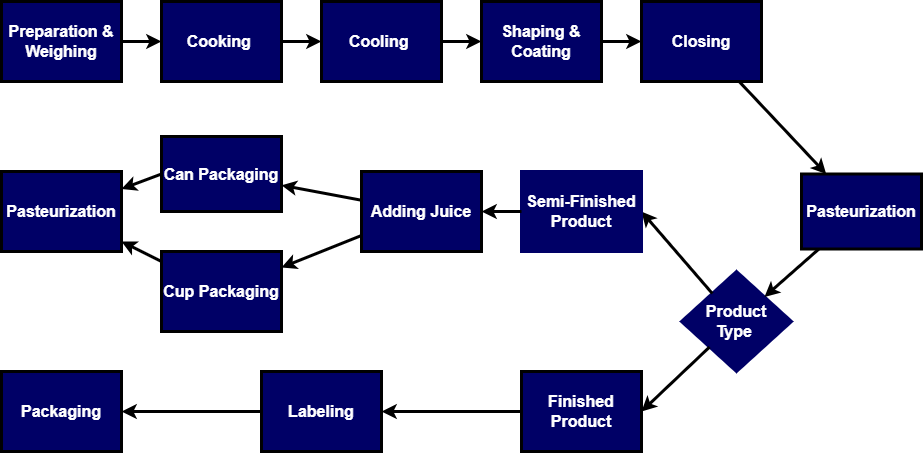
\includegraphics[width=1\linewidth]{figures/FCNew.png}
    \caption{Production workflow of popping boba in the facility}
    \label{fig:chart}
\end{figure}

\subsection{Problem Definition}
The company faced high demand during the summer season in previous years. However, it was challenging to meet this demand due to limited production capacity. The lack of storage space prevented the company from building inventory ahead, although product shelf life would allow stock to be carried over multiple months. Now that the company has transitioned to another facility, storage limitations have eased, making it essential to develop a production and inventory planning model that uses line capacity and advanced production
to meet peak-season demand. The key challenge is to balance holding and backlogging costs in terms of raw materials and produced goods. The company prepares its production plan and schedule semi-manually by evaluating market insights, past experiences, and previous demand data. Since demand levels, particularly in the domestic
market, fluctuate seasonally and cannot always be predicted precisely, a reliable and mathematically based decision support system is needed to adjust the company’s production planning accordingly. The objective of this decision support system is to generate a production plan that determines the optimal production and stocking levels of different product types, minimizing holding and backlogging costs during the high-demand season while satisfying system requirements.


\section{Literature Review}
Production planning under demand uncertainty has been the subject of sustained research for more than four decades, spanning aggregate planning, hierarchical decomposition, capacitated lot-sizing, scheduling, and stochastic programming. \cite{nahmias2015poa} present the textbook treatment of the deterministic foundation, including the trade-offs between setup, production, inventory, and backlog. The most cited modern survey of stochastic production planning is \cite{mula2006review}, which catalogs over a hundred models that incorporate demand, lead time, or capacity uncertainty and identifies aggregate production planning under uncertainty as the dominant research stream. More recent work by \cite{thevenin2021mrp} extends this tradition to multi-echelon material requirements planning (MRP) with stochastic optimization, demonstrating that jointly optimizing lot sizes and safety stocks yields substantial cost reductions over decoupled MRP heuristics. These frameworks collectively establish the cost structure, decision typology, and methodological vocabulary that our models inherit. \\
\indent At the aggregate planning level, BobaCo's long-term model belongs to the family of multi-level capacitated lot-sizing problems (MLCLSP), formally introduced by \cite{billington1983mlclsp}. The single-level capacitated lot-sizing problem (CLSP) and its variants are reviewed by \cite{karimi2003cls}, who emphasize the NP-hardness of even moderately sized instances. The multi-level extension, where intermediate items feed downstream products through a bill-of-materials, is analyzed by \cite{maes1991mlcls}, who prove that feasibility of an MLCLSP instance is itself NP-complete. The state-of-the-art exact solution approach is the fix-and-optimize heuristic of \cite{helber2010mlclsp}, which targets medium-scale instances; in our testing, a monolithic full-year daily MILP exceeded 2,200 seconds of solver time, confirming that decomposition is essential at realistic scale.\\
\indent At the operational level, our daily MILP extends beyond classical MLCLSP. Because production quantities are fully determined by binary machine-assignment variables and because Cup and Can Bubble Tea cannot share a production day, the model integrates lot-sizing decisions with daily machine-assignment scheduling. This places the operational layer in the lot-sizing and scheduling literature, surveyed by \cite{drexl1997lss}, which distinguishes pure lot-sizing problems (quantities only) from combined lot-sizing and scheduling problems (quantities, sequence, and machine assignment). The two layers of our system therefore belong to two distinct but adjacent problem classes, a distinction we exploit in the hierarchical decomposition developed in Section 4.\\
\indent The closest published structural analogs to our operational layer come from the soft drink industry. \cite{ferreira2009softdrink} formulate a mixed-integer model for a real Brazilian soft drink plant in which liquid preparation in tanks must be synchronized with parallel bottling lines, an arrangement structurally similar to our Semi-Finished Boba feeding the Cup and Can lines. \cite{toledo2009sitlsp} address the same plant with a multi-population genetic algorithm and frame it as a synchronized and integrated two-level lot-sizing and scheduling problem. \cite{turkmen2021} apply multi-stage production planning at a small food and beverage company in Türkiye. Our contribution extends these by integrating a stochastic aggregate layer with a deterministic daily scheduling layer and deploying both in a live rolling-horizon decision support system, a combination not previously published in this domain.\\
\indent A standard extension of lot-sizing models is to permit backlogging, where unmet demand is carried forward and fulfilled in a later period. The strong reformulations of \cite{PochetWolsey1988} provide the canonical reference for incorporating backlog variables and penalties into MIP lot-sizing models. We extend this framework with a two-tier penalty distinguishing regular backlog from a critical backlog beyond twelve days, the empirically observed threshold above which BobaCo's customers cancel orders. This two-tier formulation is an original modeling contribution motivated directly by industrial data.\\
\indent Hierarchical production planning (HPP) addresses the complexity of multi-period, multi-product systems by decomposing decisions across temporal aggregations. \cite{bitran1982hpp} formalize HPP as a two-stage system in which an upper-level aggregate model determines medium-term production targets that a lower-level model disaggregates into detailed schedules. \cite{liberatore1985hpp} describe an HPP system deployed at American Olean Tile, where an annual aggregate plan is linked to short-term mixed-integer scheduling and embedded in routine company practice. We follow this two-stage structure, passing monthly inventory targets from the stochastic aggregate model to the short-term scheduling MILP as hard linking constraints at days 24 and 48.\\
\indent The mathematical mechanism by which one planning level constrains another has been formalized in the capacitated lot-sizing literature. \cite{suerie2003clspl} introduce an MIP formulation in which setup and inventory variables are explicitly linked across consecutive planning periods, demonstrating that valid inequalities and decomposition heuristics can exploit this structure to achieve tight bounds. The cross-level inventory-target linking constraints we introduce at days 24 and 48 are a direct application of this principle, ensuring that the operational scheduling MILP respects the build-ahead targets identified by the stochastic aggregate model.\\
\indent Rolling-horizon execution complements hierarchical decomposition by enabling plans to be updated as new demand information becomes available. \cite{sahin2013rolling} review rolling-horizon schemes in supply chains and conclude that they are effective for maintaining responsiveness in multi-period planning, provided near-term decisions are stabilized to prevent excessive fluctuations. The stability problem itself is studied as schedule nervousness; \cite{blackburn1986nervousness} compare five nervousness-dampening strategies and prove that freezing a portion of the planning horizon dominates safety-stock and lot-for-lot approaches under most cost conditions. \cite{forel2023stochastic} extend this stream by combining stochastic lot-sizing with rolling-horizon execution, anticipating forecast updates within the stochastic formulation itself and reporting average cost reductions of fourteen percent over deterministic planning. Near-term decisions in our system are stabilized following the schedule-freezing approach of \cite{blackburn1986nervousness}, with weekly replanning aligned to the company's planning cycle.\\
\indent The stochastic aggregate layer is formulated as a two-stage stochastic program with recourse, following the textbook framework of \cite{BirgeLouveaux2011}. First-stage decisions for the first two months are made before demand uncertainty is revealed; scenario-dependent recourse decisions for months three through twelve allow production, inventory, and backlog quantities to adapt to the realized scenario. \cite{korpeoglu2011} apply a multi-stage stochastic programming approach to master production scheduling under demand and capacity uncertainty, demonstrating the value of stochastic formulations for industrial-scale planning. We follow the two-stage formulation in the aggregate layer, making first-stage decisions before uncertainty is revealed and optimizing scenario-dependent recourse over the remaining horizon.\\
\indent The benefit of solving the stochastic formulation rather than its deterministic mean-value approximation is quantified by the Value of the Stochastic Solution (VSS), formally introduced by \cite{birge1982vss} for stochastic linear programs with fixed recourse. \cite{thevenin2021mrp} compute VSS in a production planning context and confirm that the stochastic approach yields cost savings that grow with demand volatility and capacity tightness. Our 100-iteration VSS analysis applies this definition; the stochastic approach dominated the deterministic approximation in every iteration, with an average advantage of approximately 37 million Turkish lira.\\
\indent Taken together, these literature streams motivate the hierarchical stochastic rolling-horizon architecture developed in Section 4. The aggregate planning layer is a two-stage stochastic MLCLSP that determines monthly production and inventory targets. The operational layer is a multi-level lot-sizing and scheduling MILP that solves daily machine-assignment decisions subject to the aggregate-layer linking constraints. Both layers are re-solved weekly in a rolling horizon with near-term stabilization. The closest published analog, \cite{englberger2016stochastic}, integrates two-stage stochastic master production scheduling with rolling-horizon execution but does not separate the operational scheduling decisions into a distinct MILP layer with hard cross-level linking constraints. To the best of our knowledge, no prior study reports a deployed industrial decision support system that combines all three architectural elements --- a two-stage stochastic aggregate model, a separate daily operational scheduling MILP linked by explicit inventory targets, and weekly rolling-horizon execution with near-term stabilization --- in a single hierarchical stack.\\


\section{Proposed Solution Strategy}
\subsection{Problem Classification and Architectural Overview}

The planning problem faced by BobaCo spans two interconnected problem classes. At the aggregate planning level, the problem belongs to the multi-level capacitated lot-sizing problem (MLCLSP) family under demand uncertainty \citep{billington1983mlclsp, karimi2003cls, maes1991mlcls, korpeoglu2011}, where decisions concern monthly production volumes and inventory targets for a multi-level bill-of-materials with one intermediate product (Semi-Finished Boba) that is both sold directly and consumed by two finished products. At the operational scheduling level, the problem integrates lot-sizing with daily machine-assignment decisions, including a product-exclusivity constraint between Cup and Can Bubble Tea on the pasteurization line; this structure is classified by \cite{drexl1997lss} as a multi-level lot-sizing and scheduling problem. Even state-of-the-art exact methods such as the fix-and-optimize approach of \cite{helber2010mlclsp} target medium-scale instances; in our testing, a monolithic full-year daily MILP exceeded 2,200 seconds, confirming that the combined formulation is computationally intractable at planning resolution and motivating the hierarchical decomposition developed below.

\indent To the best of our knowledge, this is the first study to design, mathematically formulate, and deploy a live three-layer hierarchical decision support system that integrates a monthly two-stage stochastic aggregate planning model with a daily MILP operational scheduling model via temporal inventory-target linking constraints under a weekly rolling-horizon execution in a B2B process manufacturing setting. Existing studies address stochastic rolling-horizon planning \citep{forel2023stochastic}, integrated lot-sizing and scheduling under uncertainty \citep{drexl1997lss, ferreira2009softdrink, toledo2009sitlsp}, or stochastic multi-echelon MRP \citep{thevenin2021mrp}, but no published live industrial system combines all three architectural elements in one deployed stack \citep{englberger2016stochastic}.

\subsection{General Approach}

In order to provide a solution to the company’s challenge to satisfy demand in high-demand seasons, a production plan optimization tool with a mathematical model is required. For this purpose, an optimization model that represents the company’s production system for a full year with daily time periods had been created. Also, this model considers the operational limits of the factory, such as line-based product separation, ensuring that the proposed production and inventory plans are feasible for the real system.

\indent The main aim of this model is to plan daily production for each line and make daily inventory decisions for all products so that backlogs stay low without creating unnecessary inventory. Backlogging is allowed to preserve feasibility during temporary capacity or material shortages. However, the company does not consider backlogs within a two-week window as a critical issue, whereas delays beyond two weeks become problematic because they may lead to order cancellations. Therefore, the planning approach is designed to keep backlogs from exceeding two weeks whenever possible, while still balancing this service consideration against inventory build-up, especially under seasonal demand. 

\indent However, when this model is applied to the full year with daily detail, the problem size becomes large and difficult to solve within practical time limits. For this reason, we use a heuristic solution approach based on dividing this model into two models, namely a long-term and a short-term model. This method aims to balance solution quality and computational efficiency by generating feasible production plans that capture the system’s key constraints and objectives. 

\subsection{Critical Assumptions}
There were several critical assumptions made in order to create the models effectively and efficiently:
\begin{itemize}
    \item Semi-finished Boba and Tub Boba are two different products.
    \item Backlogging is allowed in the system.
    \item Production lines can only produce one type of product in a day.
    \item Backlogs within two weeks are treated as non-critical, while delays beyond two weeks are considered problematic and more costly due to potential order cancellations. 


\end{itemize}


\subsection{Mathematical Model}

\subsubsection{Major Constraints}
Production lines in the factory are not able to switch between products in a day. If a product is assigned to its corresponding production line, it should use it for all day. There are two production lines; the first line serves to produce boba for both Plastic Tub and Semi-Finished Boba products. Second line serves to Cup Bubble Tea and Can Bubble Tea products. Total production is limited by the workdays in that period without overtime usage. Since Semi-Finished Boba product is not directly demanded, it is used for Cup and Can products. Semi-finished Boba can also be stored for future usage of it. Other products that are not Semi-Finished Boba products are directly demanded from end customers and can be stored. There is a limited inventory area in the factory, which implies stored products' sum of usage area cannot exceed that area.
\subsubsection{Objectives}
The objective of the mathematical model is to find a long-term inventory and production strategy by minimizing holding and backlog costs to cover the high-demand season with an optimal inventory level. Corresponding costs for backlogging are relatively higher than inventory cost, so the objective function is generated to mainly find a production plan while minimizing the sum of those two costs. 
\clearpage
\subsubsection{Formulation of the Mathematical Model}
\begin{table}[h!]
\centering
\caption{Sets of Mathematical Model}
\begin{tabular}{@{}lp{11cm}@{}}
\toprule
\textbf{Sets}& \textbf{Definition} \\
\midrule
$K_1$& Set of Plastic Tub and Semi-Finished Boba Products ($K_1=\{1,2\}$)\\
$K_2$& Set of Cup Bubble Tea and Can Bubble Tea Products ($K_2=\{3,4\}$)\\
$T$& Set of Days in Period\\
$S$& Set of Raw Materials\\
$M$& Set of machines on Line 1 ($M=\{1,2,3\}$)\\
$M_3$& Set of machines for product 3 on Line 2 ($M_3=\{1,2\}$)\\
\bottomrule
\end{tabular}
\end{table}

\begin{table}[h!]
\centering
\caption{Parameters of Mathematical Model}
\begin{tabular}{@{}lp{11cm}@{}}
\toprule
\textbf{Parameters} & \textbf{Definition} \\\midrule
$b_i$& Daily unit backlog cost of product $i$\\
$b_i^{12}$& Daily unit backlog cost of product $i$ whose due date has exceeded at least 12 days\\
$n_{is}$& Number of raw material $s$ needed for one unit of product $i$\\
$LT_s$& Lead time of raw material $s$ \\
$\kappa_m$& Daily capacity of machine $m\in M$ on Line 1 (full capacity if selected)\\
$\kappa^{3}_m$& Daily capacity of machine $m\in M_3$ when producing product 3 on Line 2\\
$\kappa^{4}$& Daily capacity of Line 2 when producing product 4 (single machine)\\
$u_{23}$& Amount of product $2$ needed to produce product $3$\\
$u_{24}$& Amount of product $2$ needed to produce product $4$\\
$d_{i,t}$& Customer demand of product $i$ at day $t$\\
$h_i$& Unit holding cost of product $i$\\
$h_s^{r}$& Unit holding cost of raw material $s$ (used with weekly RM inventory)\\
$I^{max}$& Maximum inventory area \\
$v_i$& Inventory area usage of unit product $i$\\
$I_r^{max}$& Maximum raw material inventory area\\
$v_s$& Inventory area usage of unit raw material $s$\\
$w_{i,t}$& Sum of the demand obtained for product $i$ from period $t-12$ to $t$ (Demand of last 12 days)\\
$moq_s$& Minimum order quantity for raw material $s$\\
$I_{i,0}$& Initial inventory of product $i$ at the start of day 1\\
$B_{i,0}$& Initial backlog of product $i$ at the start of day 1\\
$I^{r}_{s,0}$& Initial raw material inventory of $s$ at the start of day 1\\
\bottomrule
\end{tabular}
\end{table}
\clearpage
\begin{table}[h!]
\centering
\caption{Decision Variables of Mathematical Model}
\begin{tabular}{@{}lp{11cm}@{}}
\toprule
\textbf{Variables}& \textbf{Definition} \\
\midrule
$P_{i,t}$& Number of unit $i$ produced at day $t$\\
$I_{i,t}$& Number of unit product $i$ in inventory at day $t$\\
$I_{s,t}^r$& Number of raw material $s$ in inventory at the end of day $t$\\
$R_{s,t}$& Number of raw material $s$ ordered at day $t$\\
$Z_{s,t}$& $1$ if an order is placed for raw material $s$ at day $t$, $0$ otherwise\\
$B_{i,t}$& Backlog amount of product $i$ at day $t$\\
$B_{i,t}^{12}$& Backlog amount of product $i$ at day $t$ whose due date has exceeded at least 12 days\\
$X_{m,1,t}$& $1$ if machine $m\in M$ produces product 1 at day $t$, $0$ otherwise\\
$X_{m,2,t}$& $1$ if machine $m\in M$ produces product 2 at day $t$, $0$ otherwise\\
$X_{m,3,t}$& $1$ if machine $m\in M_3$ produces product 3 at day $t$, $0$ otherwise\\
$X_{4,t}$& $1$ if Line 2 produces product 4 at day $t$, $0$ otherwise\\
\bottomrule
\end{tabular}
\end{table}

\begin{alignat}{4}
&\min && \sum_{t\in T}\sum_{i \in K_1 \cup K_2}\bigl(b_iB_{i,t}+b_i^{12}B_{i,t}^{12}+h_iI_{i,t}\bigr)
+ \sum_{t\in T}\sum_{s\in S}h^r_s I^r_{s,t} & \tag{1} \\[4pt]
&\text{s.t.} \quad
&& X_{m,1,t}+X_{m,2,t}\leq 1 && \hspace{-2cm} \forall m\in M,\forall t\in T  &\tag{2} \\[4pt]
&&& X_{m,3,t}\leq 1-X_{4,t} && \hspace{-2cm} \forall m\in M_3,\forall t\in T  &\tag{3} \\[4pt]
&&& P_{1,t}= \sum_{m\in M}\kappa_m X_{m,1,t} && \hspace{-2cm} \forall t\in T &&\tag{4}\\[4pt]
&&& P_{2,t}= \sum_{m\in M}\kappa_m X_{m,2,t} && \hspace{-2cm}\forall t\in T &&\tag{5}\\[4pt]
&&& P_{3,t}= \sum_{m\in M_3}\kappa^{3}_m X_{m,3,t} &&\hspace{-2cm} \forall t\in T &&\tag{6}\\[4pt]
&&& P_{4,t}= \kappa^{4} X_{4,t} &&\hspace{-2cm} \forall t\in T &&\tag{7}\\[4pt]
&&& I_{2,t-1}+P_{2,(t-1)}-\sum_{i\in K_2} u_{2i}P_{i,t} = I_{2,t} \quad && \hspace{-2cm} \forall t\in T &&\tag{8}\\[4pt]
&&& I_{i,t-1}+P_{i,t} - (d_{i,t}+B_{i,t-1})+B_{i,t} = I_{i,t}
&& \hspace{-2cm} \forall t\in T, \forall i\in K\backslash \{2\}  &&\tag{9}\\[4pt]
&&& I_{s,t}^{r}
= I_{s,(t-1)}^{r} + R_{s,(t-LT_s)}
-\hspace{-0.3cm}\sum_{i \in K_1 \cup K_2}\hspace{-0.3cm} n_{is}  P_{i,t}
&& \hspace{-2cm} \forall s\in S,\forall t\in T &&\tag{10}\\[4pt]
&&& R_{s,t} \ge moq_s \cdot Z_{s,t}&& \hspace{-2cm} \forall s\in S,\forall t\in T &&\tag{11}\\[4pt]
&&& I^{max} \geq \sum_{i \in K_1 \cup K_2}v_iI_{i,t} && \hspace{-2cm} \forall t\in T &&\tag{12}\\[4pt]
&&& I_r^{max} \geq \sum_{s\in S}v_sI_{s,t}^{r}&& \hspace{-2cm} \forall t\in T &&\tag{13}\\[4pt]
&&& B_{i,t}^{12} \geq B_{i,t}-w_{i,t}&& \hspace{-2cm} \forall i\in K_1 \cup K_2,\forall t\in T &&\tag{14}\\[4pt]
&&& X_{m,1,t}\in\{0,1\} ,X_{m,2,t}\in\{0,1\} &&\hspace{-2cm}  \forall m\in M, \forall t\in T &&\tag{15}\\[4pt]
&&& X_{m,3,t}\in\{0,1\},\ X_{4,t}\in\{0,1\} &&\hspace{-2cm} \forall m\in M_3,\forall t\in T &&\tag{16}\\[4pt]
&&& Z_{s,t}\in\{0,1\} &&\hspace{-2cm} \forall s\in S, \forall t\in T &&\tag{17}\\[4pt]
&&& P_{i,t},I_{i,t},B_{i,t},B_{i,t}^{12},I_{s}^r,R_{s}\geq 0
&& \hspace{-2cm} \forall i\in K,\forall t\in T, &&\tag{18}
\end{alignat}


\begin{itemize}
    \item Objective Function (1): Objective function of the Mathematical Model minimizes total holding and backlog cost.
    \item Constraints (2),(3): Enforces the updated production line structure.
    \item Constraints (4)-(7): Full-capacity production definitions based on machine selection binaries.
    \item Constraint (8): Inventory balance constraint of Semi-Finished Boba product.
    \item Constraint (9): Inventory balance constraint of finished products.
    \item Constraint (10): Weekly inventory balance constraint of raw materials (Monday orders by definition).
    \item Constraint (11): MOQ and order activation constraints.
    \item Constraints (12),(13): Inventory area limits for products and raw materials. 
    \item Constraints (14): Defines the portion of backlog older than 12 days.
    \item Constraints (15)-(18): Domain constraints for decision variables.
\end{itemize}

The two-tier backlog penalty $(B_{i,t}, B_{i,t}^{12})$ extends the standard backlogging formulation of \cite{PochetWolsey1988} by separately tracking demand unmet for more than 12 days --- the empirically observed threshold beyond which BobaCo's customers cancel orders. This two-tier structure is an original modeling contribution motivated by industrial data; it allows the model to distinguish operationally tolerable short delays from service failures with direct revenue consequences, and is reflected in the differentiated unit cost coefficients $b_i$ and $b_i^{12}$ in the objective function.


\subsection{Heuristic Approach}
In this heuristic approach, we divide the original model into two linked models: a long-term model and a short-term model. The short-term model is essentially the same mathematical model as the original one, but it is solved only for a 48-day horizon, which corresponds to the number of working days in 8 weeks. In this model, we still decide the daily production and inventory levels for each product on each line, and we add two extra parameters to incorporate long-term inventory decisions. These additional parameters come from the long-term model.

\indent The long-term model works with monthly time periods over the whole year and shows how much we plan to produce and keep in inventory at an aggregate level. To account for demand uncertainty in this planning layer, the long-term model is formulated as a two-stage stochastic program. The first stage covers the initial months (t = 1,2), where decisions are made before uncertainty is revealed. The second stage covers the remaining months (t = 3,…,12), where demand is represented through scenarios $\omega \in \Omega $ and scenario-dependent recourse decisions are optimized. The objective combines the first-stage costs with the expected second-stage costs across scenarios, and the system state at the end of t = 2 is carried into the scenario-based stage to ensure consistency.

\indent The inventory decisions obtained from this long-term model are then used as hard linking constraints in the short-term model, ensuring that the operational scheduling decisions respect the build-ahead targets identified by the stochastic aggregate model --- a coordination mechanism formalized in the capacitated lot-sizing literature by \cite{suerie2003clspl}. Both models are run in a rolling-horizon manner \citep{sahin2013rolling, forel2023stochastic}: the long-term model is solved monthly with the necessary parameter updates, and the short-term model is repeatedly solved weekly over a 2-month time period (48 workdays). Near-term decisions are stabilized following the schedule-freezing approach of \cite{blackburn1986nervousness}, which has been shown to dominate alternative nervousness-dampening strategies in rolling-horizon production planning. The combination of the two models provides a detailed short-term production schedule while still considering future demand and inventory costs. Figure \ref{fig:heur} demonstrates a chart to see the two models logic visually:
\begin{figure}[h!]
    \centering
    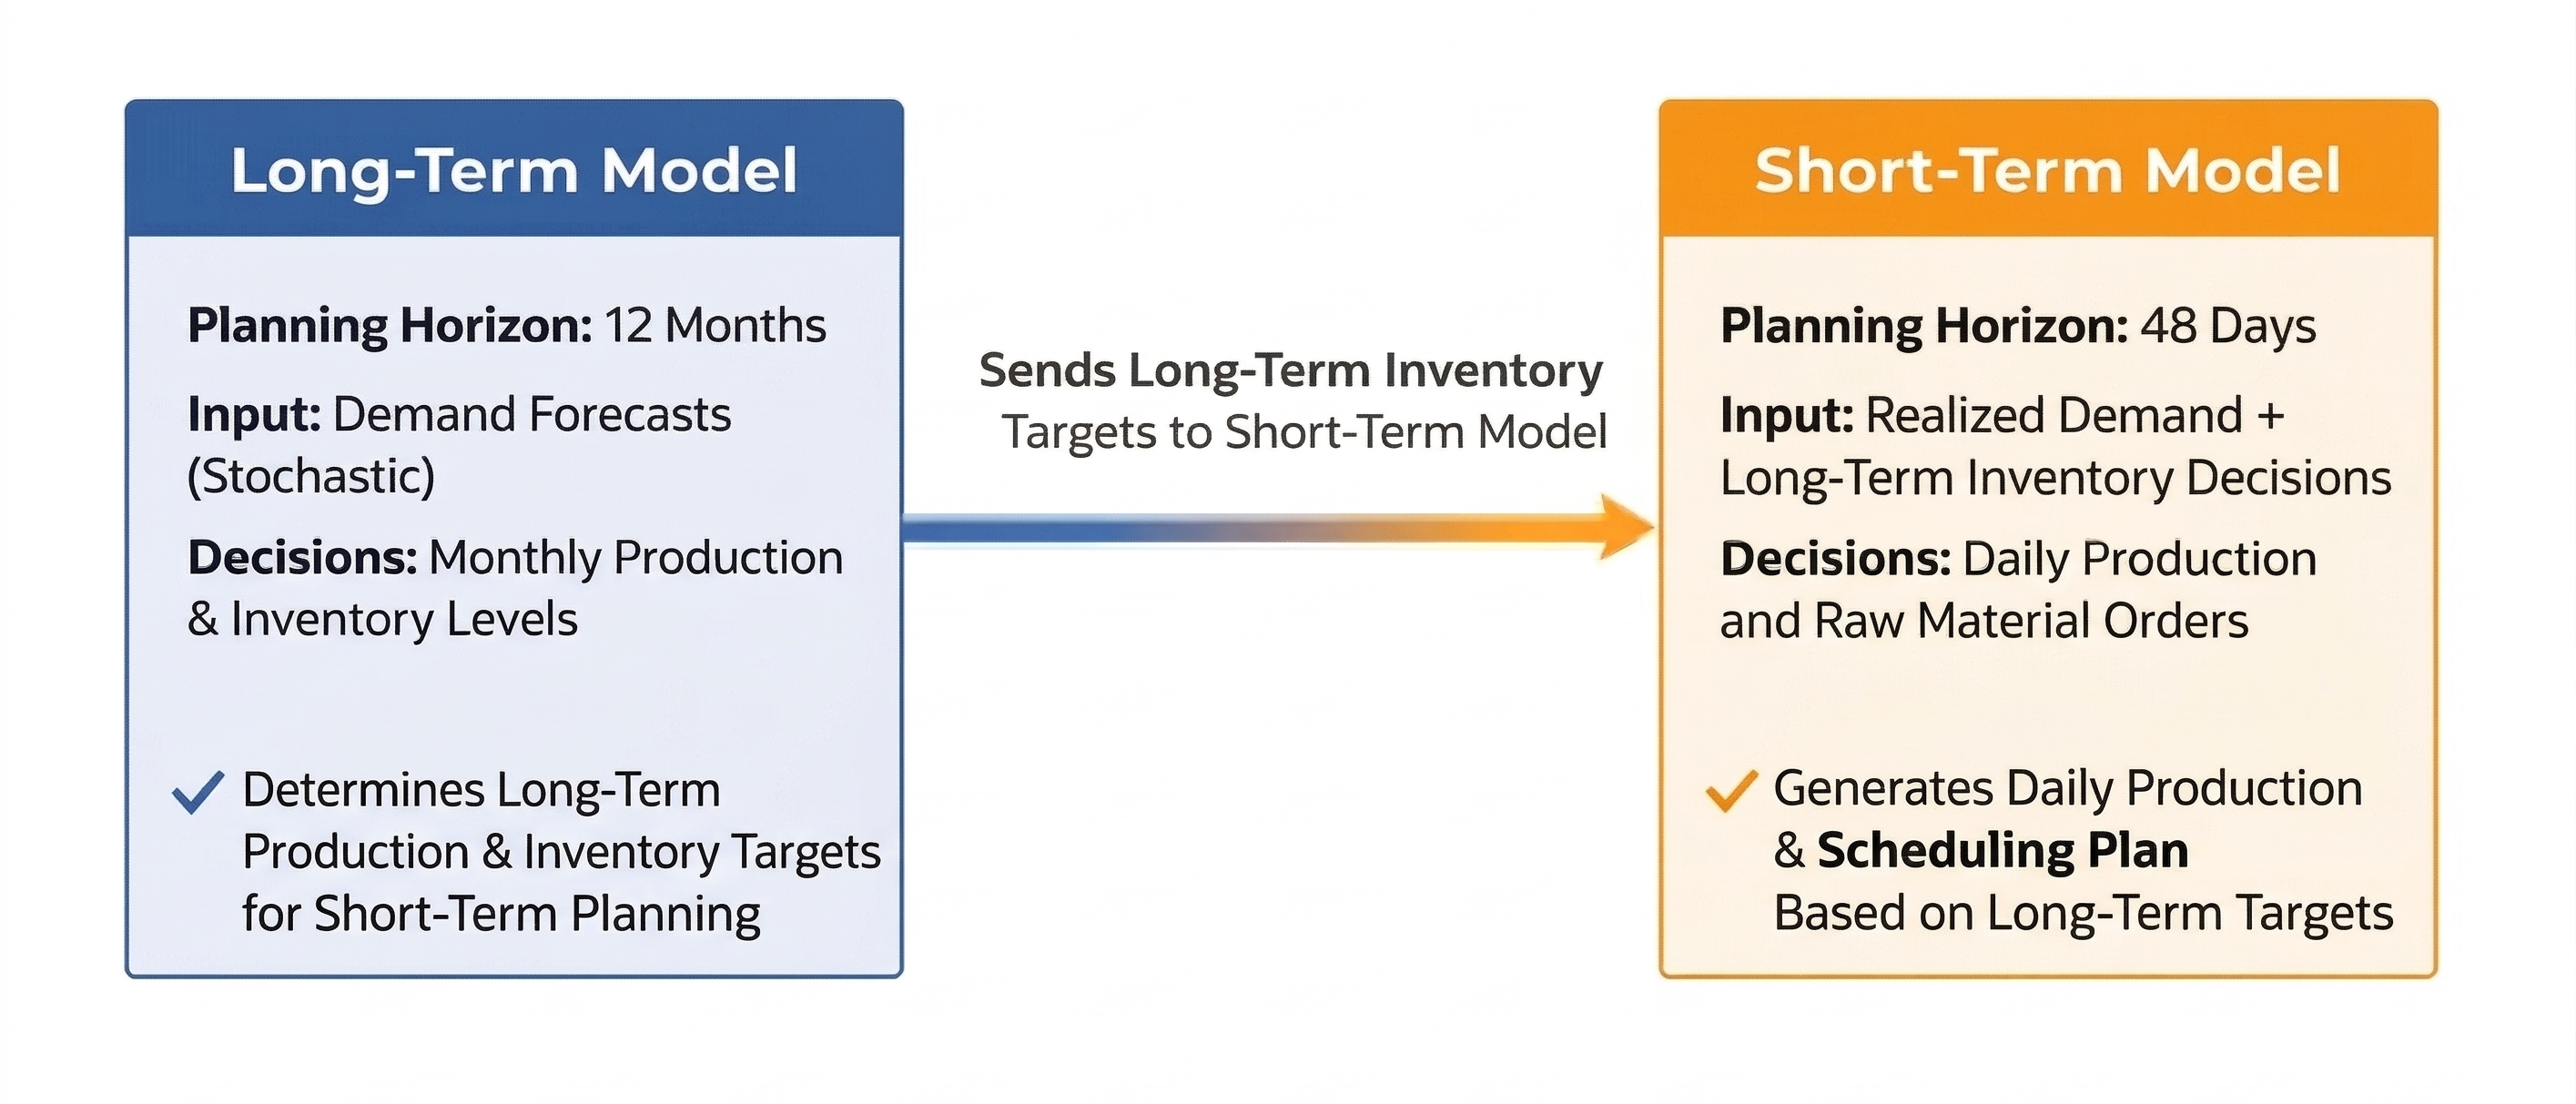
\includegraphics[width=1\linewidth]{figures/Hierarchical_models.png}
    \caption{Long-term and short-term models}
    \label{fig:heur}
\end{figure}

\subsubsection{Deterministic Long-Term Aggregate Production Planning Model}

This long-term model covers similar constraints to the mathematical model, with the exception of strict daily production capacity. Moreover, this model’s constraints cover monthly decisions and do not consider raw material existence. The objective of the long-term model is to find a less costly monthly long-term inventory strategy by minimizing holding and backlog costs to cover the high-demand season with an optimal inventory level.

\begin{table}[h!]
\centering
\caption{Sets of Deterministic Long-Term Model}
\begin{tabular}{@{}lp{11cm}@{}}
\toprule
\textbf{Sets}& \textbf{Definition} \\
\midrule
$K_1$& Set of Plastic Tub and Semi-Finished Boba Products\\
$K_2$& Set of Cup Bubble Tea and Can Bubble Tea Products\\
$T$& Set of Planning Periods ($T=\{1,\dots,12\}$)\\
$J$& Set of Production Lines\\ \bottomrule
\end{tabular}
\end{table}

\begin{table}[h!]
\centering
\caption{Parameters of Deterministic Long-Term Model}
\begin{tabular}{@{}lp{11cm}@{}}
\toprule
\textbf{Parameters} & \textbf{Definition} \\
\midrule
$d_{i,t}$& Demand of product $i$ in period $t \in \{1,2\}$\\
$a_t$& Number of workdays in period $t$\\
$b_i$& Backlog cost for product $i$\\
$c_1$& Daily unit capacity of production line 1\\
$c_{2,i}$& Daily unit capacity of production line 2 for product $i$\\
$I^{max}$& Maximum storage area\\
$r_i$& Unit usage area of product $i$\\
$u_{i2}$& Number of product 2 used in the production of product $i\in \{3,4\}$\\
$h_i$& Holding cost of product $i$ for unit period\\
\bottomrule
\end{tabular}
\end{table}
\vspace{10.0em}
\begin{table}[h!]
\centering
\caption{Decision Variables of Deterministic Long-Term Model}
\begin{tabular}{@{}lp{11cm}@{}}
\toprule
\textbf{Variables}& \textbf{Definition} \\
\midrule
$P_{i,t}$& Production amount of product $i$ at period $t \in \{1,2\}$ \\
$I_{i,t}$& Inventory amount of product $i$ at the end of period $t \in \{1,2\}$\\
$B_{i,t}$& Backlog amount of product $i$ at period $t \in \{1,2\}$\\ \bottomrule
\end{tabular}
\end{table}

\begin{alignat}{4}
&\min && \sum_{t=1}^{2}\sum_{i \in K_1 \cup K_2}\bigl(b_iB_{i,t}+h_iI_{i,t}\bigr)
&& \tag{1} \\[4pt]
&\text{s.t.} \quad
&& \sum_{i \in K_1}\frac{P_{i,t}}{c_1} \leq a_t  && \forall t\in \{1,2\} &&\tag{2}\\[4pt]
&&& \sum_{i \in K_2}\frac{P_{i,t}}{c_{2,i}}  \leq a_t  && \forall t\in \{1,2\} &&\tag{3}\\[4pt]
&&& I_{2,t-1}+P_{2,t}-\sum_{i\in K_2}u_{i2}\,P_{i,t} = I_{2,t} \quad && \forall t\in \{1,2\} &&\tag{4}\\[4pt]
&&& I_{i,t-1}+P_{i,t} - (d_{i,t}+B_{i,t-1})+B_{i,t} = I_{i,t}
&&  &&\tag{5}\\[4pt]
&&& && \hspace{-2cm} \forall t\in \{1,2\},\forall i\in (K_1 \cup K_2)\backslash \{2\} &&\tag{5}\\
&&& I^{max} \geq \sum_{i=1}^{4} r_i I_{i,t} && \forall t\in \{1,2\} &&\tag{6}\\[4pt]
&&& P_{i,t},I_{i,t},B_{i,t} \geq 0
&& \forall i\in K_1 \cup K_2,\forall t\in T
&&\tag{7}
\end{alignat}

\begin{itemize}
    \item \textbf{Objective Function (1):} The objective function of the deterministic long-term model minimizes the total holding and backlog costs over the deterministic planning horizon.
    \item \textbf{Constraints (2)-(3):} These constraints represent the production capacity limitations of the two production lines. Constraint (2) restricts the total production assigned to line 1 by the number of available workdays in period $t$, while Constraint (3) imposes the same limitation for line 2.
    \item \textbf{Constraint (4):} This constraint is the inventory balance equation for Semi-Finished Boba (product 2). It states that the ending inventory of product 2 equals the beginning inventory plus production minus the quantity used as an input in the production of products in set $K_2$.
    \item \textbf{Constraint (5):} This is the inventory--backlog balance constraint. It ensures that, for each product and period, available inventory and production are allocated between demand fulfillment, backlog carryover, and ending inventory.
    \item \textbf{Constraint (6):} This constraint enforces the storage capacity limitation by ensuring that the total area occupied by end-of-period inventory does not exceed the maximum available storage area.
    \item \textbf{Constraint (7):} This constraint imposes non-negativity on the production, inventory, and backlog decision variables.
\end{itemize}



\subsubsection{Two-Stage Stochastic Long-Term Aggregate Production Planning Model}
To include demand uncertainty in the solution approach, the long-term model is formulated as a two-stage stochastic program with recourse \citep{BirgeLouveaux2011}, where first-stage production and inventory decisions for the early months are fixed before uncertainty is revealed and second-stage recourse decisions adapt to the realized demand scenario in the remaining months. Multi-stage stochastic programming applications to master production scheduling under demand uncertainty are surveyed by \cite{korpeoglu2011} and \cite{thevenin2021mrp}.

\begin{table}[h!]
\centering
\caption{Sets of Long-Term Model}
\begin{tabular}{@{}lp{11cm}@{}}
\toprule
\textbf{Sets}& \textbf{Definition} \\
\midrule
$K_1$& Set of Plastic Tub and Semi-Finished Boba Products\\
$K_2$& Set of Cup Bubble Tea and Can Bubble Tea Products\\
$T$& Set of Planning Periods ($T=\{1,\dots,12\}$)\\
$J$& Set of Production Lines\\
$\Omega$& Set of Scenarios\\
\bottomrule
\end{tabular}
\end{table}
\clearpage
\begin{table}[h!]
\centering
\caption{Parameters of Long-Term Model}
\begin{tabular}{@{}lp{11cm}@{}}
\toprule
\textbf{Parameters} & \textbf{Definition} \\
\midrule
$d_{i,t}$& Demand of product $i$ in period $t \in \{1,2\}$\\
$d_{i,t,\omega}$& Demand of product $i$ in period $t \in \{3,4,\dots,12\}$ under scenario $\omega$\\
$a_t$& Number of workdays in period $t$\\
$b_i$& Backlog cost for product $i$\\
$c_1$& Daily unit capacity of production line 1\\
$c_{2,i}$& Daily unit capacity of production line 2 for product $i$\\
$I^{max}$& Maximum storage area\\
$r_i$& Unit usage area of product $i$\\
$u_{i2}$& Number of product 2 used in the production of product $i\in \{3,4\}$\\
$h_i$& Holding cost of product $i$ for unit period\\
\bottomrule
\end{tabular}
\end{table}

\begin{table}[h!]
\centering
\caption{Decision Variables of Long-Term Model}
\begin{tabular}{@{}lp{11cm}@{}}
\toprule
\textbf{Variables}& \textbf{Definition} \\
\midrule
$P_{i,t}$& Production amount of product $i$ at period $t \in \{1,2\}$ \\
$I_{i,t}$& Inventory amount of product $i$ at the end of period $t \in \{1,2\}$\\
$B_{i,t}$& Backlog amount of product $i$ at period $t \in \{1,2\}$\\
$P_{i,t,\omega}$& Production amount of product $i$ at period $t$ under scenario $\omega$\\
$I_{i,t,\omega}$& Inventory amount of product $i$ at the end of period $t$ under scenario $\omega$\\
$B_{i,t,\omega}$& Backlog amount of product $i$ at period $t$ under scenario $\omega$\\
\bottomrule
\end{tabular}
\end{table}


\newpage
\begin{alignat}{4}
&\min && \sum_{t=1}^{2}\sum_{K_1 \cup K_2}\bigl(b_iB_{i,t}+h_iI_{i,t}\bigr)
+ \sum_{\omega\in\Omega}\sum_{t=3}^{12}\sum_{i \in K_1 \cup K_2}{p_{\omega}}\bigl(b_iB_{i,t,\omega}+h_iI_{i,t,\omega}\bigr)
&& \tag{1} \\[4pt]
&\text{s.t.} \quad
&& \sum_{i \in K_1}\frac{P_{i,t}}{c_1} \leq a_t  && \hspace{-4cm} \forall t\in \{1,2\} &&\tag{2}\\[4pt]
&&& \sum_{i \in K_2}\frac{P_{i,t}}{c_{2,i}}  \leq a_t  &&\hspace{-4cm}  \forall t\in \{1,2\} &&\tag{3}\\[4pt]
&&& \sum_{i \in K_1}\frac{P_{i,t,\omega}}{c_1} \leq a_t  && \hspace{-4cm}\forall t\in \{3,12\},\forall \omega \in \Omega &&\tag{4}\\[4pt]
&&& \sum_{i \in K_2} \frac{P_{i,t,\omega}}{c_{2,i}} \leq a_t  && \hspace{-4cm}\forall t\in \{3,12\},\forall \omega \in \Omega &&\tag{5}\\[4pt]
&&& I_{2,t-1}+P_{2,t}-\sum_{i\in K_2}u_{i2}\,P_{i,t} = I_{2,t} \quad &&\hspace{-4cm} \forall t\in \{1,2\} &&\tag{6}\\[4pt]
&&& I_{2,2}+P_{2,3,\omega}-\sum_{i\in K_2}u_{i2}\,P_{i,3,\omega} = I_{2,3,\omega} \quad && \hspace{-4cm} \forall \omega \in \Omega &&\tag{7}\\[4pt]
&&& I_{2,t-1,\omega}+P_{2,t,\omega}-\sum_{i\in K_2}u_{i2}\,P_{i,t,\omega} = I_{2,t,\omega} \quad && \hspace{-4cm} \forall t\in \{4,\dots,12\} &&\tag{8}\\[4pt]
&&& I_{i,t-1}+P_{i,t} - (d_{i,t}+B_{i,t-1})+B_{i,t} = I_{i,t}
&&  &&\tag{9}\\[4pt]
&&& && \hspace{-6cm} \forall t\in \{1,2\},\forall i\in (K_1 \cup K_2)\backslash \{2\} &&\tag{9}\\[4pt]
&&& I_{i,2}+P_{i,3,\omega} - (d_{i,3,\omega}+B_{i,2})+B_{i,3,\omega} = I_{i,3,\omega}
&&  &&\tag{10}\\[4pt]
&&& && \hspace{-6cm} \forall \omega \in \Omega,\forall i\in (K_1 \cup K_2)\backslash \{2\}&&\tag{10}\\[4pt]
&&& I_{i,t-1,\omega}+P_{i,t,\omega} - (d_{i,t,\omega}+B_{i,t-1,\omega})+B_{i,t,\omega} = I_{i,t,\omega}
&& &&\tag{11}\\[4pt]
&&& && \hspace{-9cm} \forall t\in \{4,\dots,12\},\forall \omega \in \Omega,\forall i\in (K_1 \cup K_2)\backslash \{2\} &&\tag{11}\\[4pt]
&&& I^{max} \geq \sum_{i=1}^{4} r_i I_{i,t} && \hspace{-4cm}\forall t\in \{1,2\} &&\tag{12}\\[4pt]
&&& I^{max} \geq \sum_{i=1}^{4} r_i I_{i,t,\omega} && \hspace{-5cm}\forall t\in \{3,\dots,12\},\forall \omega\in\Omega &&\tag{13}\\[4pt]
&&& P_{i,t},I_{i,t},B_{i,t},P_{i,t,\omega},I_{i,t,\omega},B_{i,t,\omega} \geq 0
&&  &&\tag{14}\\
&&& && \hspace{-6cm}\forall i\in K_1 \cup K_2,\forall t\in T,\forall \omega \in \Omega &&\tag{14} 
\end{alignat}

\begin{itemize}
    \item Objective Function (1): Objective function of the long-term model minimizes total yearly holding and backlog costs.
    \item Constraints (2)-(5): Enforcing that the production amount doesn't exceed production capacity.
    \item Constraints (6)-(8): Inventory balance constraints of Semi-Finished Boba product (product 2).
    \item Constraints (9)-(11): Inventory balance constraints of finished products.
    \item Constraints (12)-(13): Ensures that total used inventory area doesn't exceed maximum inventory area.
    \item Constraint (14): Non-negativity constraint of decision variables.
\end{itemize}



\subsubsection{Scenario Generation for the Two-Stage Long-Term Model}
\label{sec:scenario_generation}

The decision support system performs production planning over a one-year horizon while treating the first two months of demand as known inputs. The purpose is to represent demand uncertainty in a controlled way and to avoid relying on a single forecast path. We do not build an internal forecasting model because demand is highly uncertain and reliable historical demand data are not available. Instead, the system receives a user-provided forecast vector and transforms it into a set of demand scenarios for the two-stage stochastic programming formulation. Therefore, the forecast is treated as the mean demand level, and uncertainty is introduced through scenario sampling around this mean.

\indent Let $f_{1},\ldots,f_{10}$ denote the company-provided forecasts for the uncertain months, corresponding to months $3$ to $12$ of the planning horizon, and let $s_{1},\ldots,s_{10}$ denote the monthly deviation rates specified by the company. Each $s_t$ is interpreted as the maximum relative deviation around the forecast mean for month $t$. The objective of the scenario generator is to create $N$ plausible $10$-month demand paths, each representing one realization of uncertainty in the second-stage horizon, while guaranteeing that every monthly value stays within the uncertainty band defined by the company.

\indent For each month $t \in \{1,\ldots,10\}$, lower and upper bounds are defined as
\begin{align}
L_t &= f_t(1 - s_t), \\
U_t &= f_t(1 + s_t).
\end{align}

\indent A demand scenario is generated by sampling uniformly within these bounds:
\begin{align}
D_{k,t} &= L_t + u_{k,t}\bigl(U_t - L_t\bigr), \qquad u_{k,t} \sim \mathrm{Uniform}(0,1).
\end{align}

\indent By construction, $D_{k,t} \in [L_t, U_t]$ for all scenarios $k$ and months $t$. For integration, months $1$--$2$ are treated as deterministic inputs and remain fixed, while the scenario generator is applied only to months $3$--$12$. Each generated vector $(D_{k,1},\ldots,D_{k,10})$ is then used as the scenario-specific demand realization in the stochastic formulation by indexing uncertain-month demand with $k$. All demand-driven constraints and cost terms in the second-stage horizon are evaluated separately for each scenario using its own $D_{k,t}$ values, and the overall objective aggregates these scenario outcomes using scenario probabilities. When no additional information is available, equal probabilities are assigned, so $p_k = 1/N$, and the model minimizes the expected total cost across the scenario set.


\subsubsection{Short-Term Production Planning Model}

This model is a shortened version of the Main Mathematical Model, with the additional two parameters introduced. These new parameters are the necessary inventory decisions obtained from the Long-Term Model. The model tries to satisfy these inventory decisions until the given days of these parameters.

\indent The objective of the short-term model is to satisfy both yearly production decisions that came from the long-term model and the realized demand in an 8-week period.  In order to generate an accurate and efficient production plan, a mixed integer linear planning model is created. This model aims to get the necessary inventory decisions from the long-term model and find a near-optimal production schedule to satisfy them. \\

\begin{table}[h!]
\centering
\caption{Sets of Short-Term Model}
\begin{tabular}{@{}lp{11cm}@{}}
\toprule
\textbf{Sets}& \textbf{Definition} \\
\midrule
$K_1$& Set of Plastic Tub and Semi-Finished Boba Products ($K_1=\{1,2\}$)\\
$K_2$& Set of Cup Bubble Tea and Can Bubble Tea Products ($K_2=\{3,4\}$)\\
$T$& Set of Days in Period\\
$S$& Set of Raw Materials\\
$M$& Set of machines on Line 1 ($M=\{1,2,3\}$)\\
$M_3$& Set of machines for product 3 on Line 2 ($M_3=\{1,2\}$)\\
\bottomrule
\end{tabular}
\end{table}

\begin{table}[h!]
\centering
\caption{Parameters of Short-Term Model}
\begin{tabular}{@{}lp{11cm}@{}}
\toprule
\textbf{Parameters} & \textbf{Definition} \\\midrule
$b_i$& Daily unit backlog cost of product $i$\\
$b_i^{12}$& Daily unit backlog cost of product $i$ whose due date has exceeded at least 12 days\\
$n_{is}$& Number of raw material $s$ needed for one unit of product $i$\\
$LT_s$& Lead time of raw material $s$ \\
$\kappa_m$& Daily capacity of machine $m\in M$ on Line 1 (full capacity if selected)\\
$\kappa^{3}_m$& Daily capacity of machine $m\in M_3$ when producing product 3 on Line 2\\
$\kappa^{4}$& Daily capacity of Line 2 when producing product 4 (single machine)\\
$u_{23}$& Amount of product $2$ needed to produce product $3$\\
$u_{24}$& Amount of product $2$ needed to produce product $4$\\
$d_{i,t}$& Customer demand of product $i$ at day $t$\\
$d^D_{i,1} , d^D_{i,2}$& Long-term inventory decision parameters\\
$h_i$& Unit holding cost of product $i$\\
$h_s^{r}$& Unit holding cost of raw material $s$ (used with weekly RM inventory)\\
$I^{max}$& Maximum inventory area \\
$v_i$& Inventory area usage of unit product $i$\\
$I_r^{max}$& Maximum raw material inventory area\\
$v_s$& Inventory area usage of unit raw material $s$\\
$w_{i,t}$& Sum of the demand obtained for product $i$ from period $t-12$ to $t$ (Demand of last 12 days)\\
$moq_s$& Minimum order quantity for raw material $s$\\
$I_{i,0}$& Initial inventory of product $i$ at the start of day 1\\
$B_{i,0}$& Initial backlog of product $i$ at the start of day 1\\
$I^{r}_{s,0}$& Initial raw material inventory of $s$ at the start of day 1\\
\bottomrule
\end{tabular}
\end{table}
\clearpage
\begin{table}[h!]
\centering
\caption{Decision Variables of Short-Term Model}
\begin{tabular}{@{}lp{11cm}@{}}
\toprule
\textbf{Variables}& \textbf{Definition} \\
\midrule
$P_{i,t}$& Number of unit $i$ produced at day $t$\\
$I_{i,t}$& Number of unit product $i$ in inventory at day $t$\\
$I_{s,t}^r$& Number of raw material $s$ in inventory at the end of day $t$\\
$R_{s,t}$& Number of raw material $s$ ordered at day $t$\\
$Z_{s,t}$& $1$ if an order is placed for raw material $s$ at day $t$, $0$ otherwise\\
$B_{i,t}$& Backlog amount of product $i$ at day $t$\\
$B_{i,t}^{12}$& Backlog amount of product $i$ at day $t$ whose due date has exceeded at least 12 days\\

\bottomrule
\end{tabular}
\end{table}

\begin{alignat}{4}
&\min && \sum_{t\in T}\sum_{i \in K_1 \cup K_2}\bigl(b_iB_{i,t}+b_i^{12}B_{i,t}^{12}+h_iI_{i,t}\bigr)
+ \sum_{t\in T}\sum_{s\in S}h^r_s I^r_{s,t}
&& \tag{1} \\[4pt]
&\text{s.t.} \quad
&& X_{m,1,t}+X_{m,2,t}\leq 1 &&  \hspace{-2cm}\forall m\in M,\forall t\in T  &&\tag{2} \\[4pt]
&&& X_{m,3,t}\leq 1-X_{4,t} && \hspace{-2cm}\forall m\in M_3,\forall t\in T  &&\tag{3} \\[4pt]
&&& P_{1,t}= \sum_{m\in M}\kappa_m X_{m,1,t} && \hspace{-2cm}\forall t\in T &&\tag{4}\\[4pt]
&&& P_{2,t}= \sum_{m\in M}\kappa_m X_{m,2,t} && \hspace{-2cm}\forall t\in T &&\tag{5}\\[4pt]
&&& P_{3,t}= \sum_{m\in M_3}\kappa^{3}_m X_{m,3,t} &&\hspace{-2cm} \forall t\in T &&\tag{6}\\[4pt]
&&& P_{4,t}= \kappa^{4} X_{4,t} &&\hspace{-2cm} \forall t\in T &&\tag{7}\\[4pt]
&&& I_{2,t-1}+P_{2,(t-1)}-\sum_{i\in K_2} u_{2i}P_{i,t} = I_{2,t} \quad &&\hspace{-2cm} \forall t\in T &&\tag{8}\\[4pt]
&&& I_{i,t-1}+P_{i,t} - (d_{i,t}+B_{i,t-1})+B_{i,t} = I_{i,t}
&& \hspace{-2cm}\forall t\in T, \forall i\in (K_1 \cup K_2)\backslash \{2\}  &&\tag{9}\\[4pt]
&&& I_{s,t}^{r}
= I_{s,(t-1)}^{r} + R_{s,(t-LT_s)}
-\sum_{i \in K_1 \cup K_2} n_{is}P_{i,t}
&& \hspace{-2cm}\forall s\in S,\forall t\in T &&\tag{10}\\[4pt]
&&& R_{s,t} \ge moq_s \cdot Z_{s,t}&&\hspace{-2cm} \forall s\in S,\forall t\in T &&\tag{11}\\[4pt]
&&& I^{max} \geq \sum_{i \in K_1 \cup K_2}v_iI_{i,t} &&\hspace{-2cm} \forall t\in T &&\tag{12}\\[4pt]
&&& I_r^{max} \geq \sum_{s\in S}v_sI_{s,t}^{r}&&\hspace{-2cm} \forall t\in T &&\tag{13}\\[4pt]
&&& B_{i,t}^{12} \geq B_{i,t}-w_{i,t}&&\hspace{-2cm} \forall i\in K_1 \cup K_2,\forall t\in T &&\tag{14}\\[4pt]
&&& I_{i,24} \geq d_{i,1}^D&&\hspace{-2cm} \forall i\in K_1 \cup K_2&&\tag{15}\\[4pt]
&&& I_{i,48} \geq d_{i,2}^D&& \hspace{-2cm}\forall i\in K_1 \cup K_2&&\tag{16}\\[4pt]
&&& X_{m,1,t}\in\{0,1\} ,X_{m,2,t}\in\{0,1\} &&\hspace{-2cm} \forall m\in M, \forall t\in T &&\tag{17}\\[4pt]
&&& X_{m,3,t}\in\{0,1\},\ X_{4,t}\in\{0,1\} && \hspace{-2cm}\forall m\in M_3,\forall t\in T &&\tag{18}\\[4pt]
&&& Z_{s,t}\in\{0,1\} &&\hspace{-2cm} \forall s\in S, \forall t\in T &&\tag{19}\\[4pt]
&&& P_{i,t},I_{i,t},B_{i,t},B_{i,t}^{12},I_{s}^r,R_{s}\geq 0
&&\hspace{-2cm} \forall i\in K_1 \cup K_2,\forall t\in T,\forall s\in S &&\tag{20}
\end{alignat}



\begin{itemize}
    \item Objective Function (1): Objective function of the Short-Term Mathematical Model minimizes total holding and backlog cost.
    \item Constraints (2),(3): Enforces the updated production line structure.
    \item Constraints (4)-(7): Full-capacity production definitions based on machine selection binaries.
    \item Constraint (8): Inventory balance constraint of Semi-Finished Boba product.
    \item Constraint (9): Inventory balance constraint of finished products.
    \item Constraint (10): Weekly inventory balance constraint of raw materials (Monday orders by definition).
    \item Constraint (11): MOQ and order activation constraints.
    \item Constraints (12),(13): Inventory area limits for products and raw materials. 
    \item Constraints (15),(16): Satisfaction of long-term inventory targets at days 24 and 48.
    \item Constraints (17)-(20): Domain constraints for decision variables.
\end{itemize}


\subsection{Verification}
\subsubsection{Verification of the Mathematical Model}

The verification procedure was conducted to assess the internal validity, logical consistency, and computational behavior of the mathematical model under systematically altered operational conditions. The model was exposed to a series of controlled test cases and to nine demand scenarios exhibiting progressively stronger seasonality and variation. The objective of this verification was twofold: (i) to ensure that the structural relations embedded within the model behave in accordance with theoretical expectations, and (ii) to evaluate the scalability and computational limits of the exact optimization framework.\\

\textbf{Logical Verification via Structured Test Cases}\\

\textbf{\indent CASE I – Cost Symmetry (BC = HC)}: When backlog and holding costs are identical, the model becomes indifferent between inventory accumulation and backlogging. The resulting production plan is concentrated near the demand period, which is a rational outcome given the large demand volumes.\\

\textbf{CASE II – Backlog-Dominant Regime (BC $>$ HC)}: For all tested ratios, the model advances production to earlier periods to avoid high backlog penalties. The monotonic relationship between increasing backlog cost and earlier production onset verifies the correct functioning of the cost–time trade-off mechanism.\\

\textbf{CASE III – Holding-Dominant Regime (HC $>$ BC):} When holding costs exceed backlog costs, the model systematically delays production until the latest feasible period. Inventory levels remain near zero, demonstrating that the model minimizes inventory exposure as predicted by cost theory.\\

\textbf{CASE IV – No Initial Raw Materials}: Production is deferred until the first arrival of raw materials. Immediately upon availability, the model initiates production. This confirms the correct modeling of dependency constraints between raw material inventories and production decisions.\\

\textbf{CASE V – High Raw Material Holding Cost:}When raw material holding cost surpasses backlog cost, the model avoids storing raw materials and consumes them immediately once available. This confirms correct economic prioritization on the upstream inventory level.\\

\textbf{CASE VI – Single-Product Demand:}Both moderate and extremely large demand configurations yield stable and theoretically consistent production patterns. This indicates robustness when dimensionality is reduced.\\

\textbf{CASE VII – Universally High Demand:}The model retains feasibility and structural consistency even under extreme demand loads, demonstrating that the formulation scales correctly with respect to demand magnitude.\\

\textbf{CASE VIII – Universally Low Demand:}The model produces a backlog-free plan and operates with minimal inventory, confirming that the constraints are flexible and that the model properly adjusts to low-pressure environments.\\

\textbf{CASE IX – Near-Zero Raw Material Lead Times:}This case resulted in markedly elevated computational times. The collapse of temporal separation between material arrival and production increases the density of feasible decision interactions, thereby expanding the search space. The resulting computational burden is indicative of a structural sensitivity to lead-time reductions.\\

\textbf{Scenario-Based Verification: Increasing Seasonality and Randomness in Demand} \\


The nine demand scenarios were constructed such that seasonality and random fluctuations intensify monotonically from Scenario 1 to Scenario 9. The computational performance exhibits a clear nonlinear pattern:

\begin{itemize}
    \item Scenarios 1–7 were solved rapidly and reliably. However, computation times still increase regarding randomness.
    \item Scenario 8 shows a pronounced increase in computational effort.
    \item Scenario 9 produces a dramatic escalation in runtime, exceeding 2200 seconds.

\end{itemize}
This progression indicates that increasing stochasticity and seasonal clustering significantly enlarge the feasible region, intensify intertemporal constraints, and consequently reduce solver efficiency. Although the model remains feasible across all scenarios, the computational cost exhibits quasi-exponential growth as demand irregularity increases.\\

\textbf{Rationale for Employing a Heuristic Approach}\\

While the exact optimization model demonstrates strong internal validity and consistent logical behavior across all controlled cases, the verification process also reveals a fundamental limitation: the exact solution does not scale computationally under high-seasonality, high-randomness, or densely coupled lead-time conditions. As seasonality intensifies, production and inventory decisions become more interdependent across time, enlarging the solution space at a faster-than-linear rate.

\begin{itemize}
    \item Very short lead times compress the problem temporally, causing decision layers that were previously sequential to become simultaneous, thereby increasing solver difficulty.
    \item The observed spike in runtime from Scenario 7 to Scenario 9 empirically confirms that exact methods exhibit near-exponential increases in computational effort under realistic stochastic demand conditions.


\end{itemize}

\begin{figure}[h!]
    \centering
    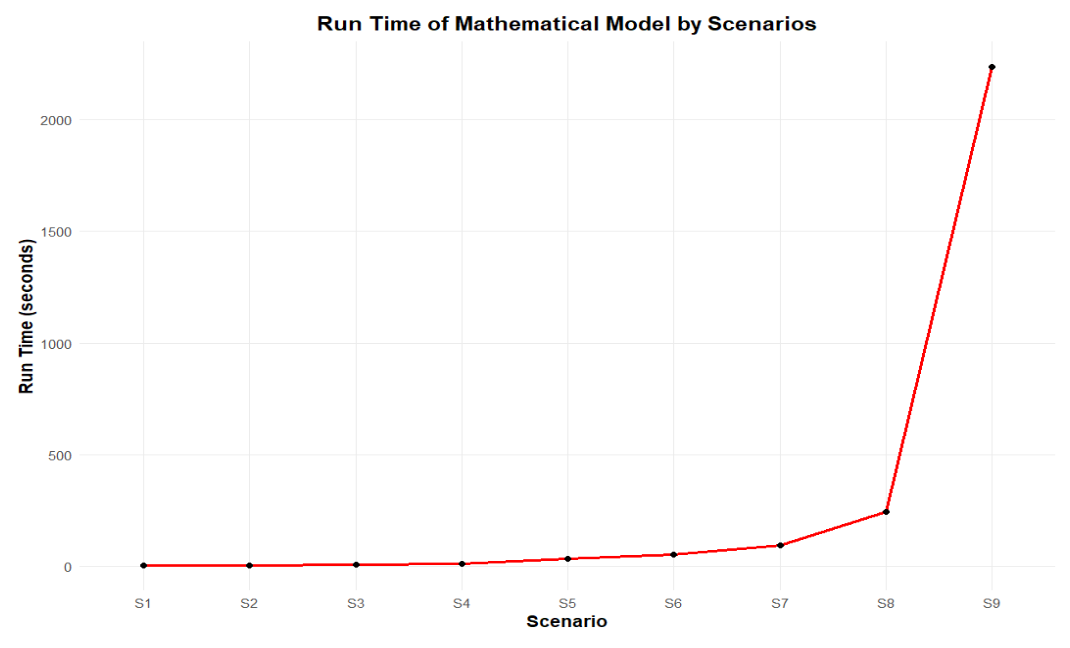
\includegraphics[width=0.9\linewidth]{figures/Draft_Model_runtime.png}
    \caption{Runtime of the Mathematical Model by Scenarios}
    \label{fig:placeholder}
\end{figure}
\begin{figure}[h!]
    \centering
    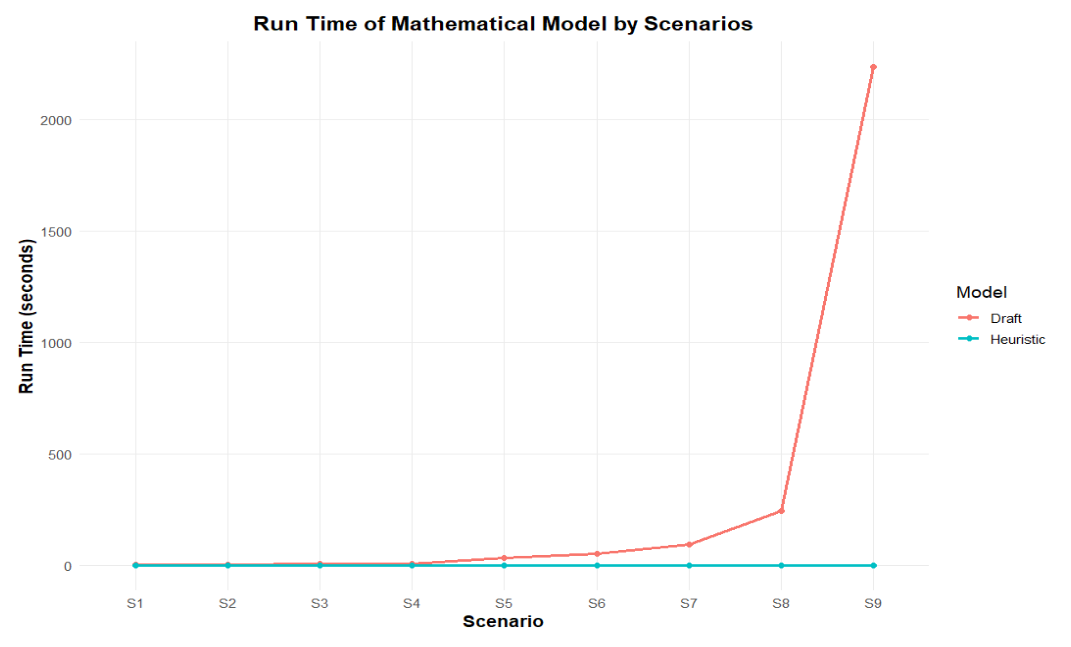
\includegraphics[width=0.9\linewidth]{figures/Model_runtime_comparison.png}
    \caption{Run Times of the Mathematical Model and Heuristic Approach by Scenario}
    \label{fig:placeholder}
\end{figure}
For these reasons, adopting a heuristic methodology becomes not merely advantageous but methodologically necessary. A heuristic approach can generate high-quality solutions within bounded and predictable time limits, and bypass exhaustive search procedures that dominate exact solvers under complex conditions. Also, it can enable long-term horizon simulations that would otherwise be computationally prohibitive.



\subsubsection{Verification of the Hierarchical Heuristic}

To assess the reliability of the rolling horizon heuristic, the exact solution and the heuristic were run over a full-year horizon under the same demand patterns. Since the heuristic is hierarchical and state-dependent, it was executed iteratively: the long-term plan was re-optimized every four weeks, the short-term plan was re-optimized weekly, and the resulting production and inventory states were carried forward to the next iteration. As the heuristic approaches the end of the year, periods that fall outside the remaining planning window are treated as having zero demand, which is a standard rolling-horizon convention and may create mild end-of-horizon effects.

\indent When comparing the heuristic against the exact solution across demand patterns, three performance indicators were tracked: total objective value, the amount of backlog exceeding ten days, and average lateness per unit. The average lateness per unit is reported as a demand-normalized measure, which allows comparison across scenarios with different total order volumes.

\indent In demand patterns where the annual load is below capacity and demand is not strongly clustered, the heuristic behaves close to the exact solution in terms of long-overdue backlog. In these settings, backlog exceeding ten days is typically absent. In the few cases where it appears, it remains very small relative to total annual orders. Although the heuristic may generate higher short-lived backlog totals than the exact solution, this difference mainly translates into small changes in average lateness per unit. Across the below-capacity scenarios evaluated, the objective deviation did not exceed approximately 20 percent, and the increase in average lateness per unit remained below roughly half a day.

\indent As demand approaches capacity, all three indicators reach their highest levels among the realistic scenarios. In the most tightly loaded cases, backlog exceeding ten days becomes nonzero for the heuristic and corresponds to roughly a few days of production volume. However, in the observed results this quantity did not exceed about 0.1 percent of total annual orders. In these same cases, the average lateness per unit remains interpretable: the heuristic increases short-lived backlog compared to the benchmark, but the implied average lateness stays within a limited range rather than escalating to persistent congestion.

\indent In demand patterns that exceed capacity and exhibit heavy clustering, backlog exceeding ten days increases for both methods. Relative to the exact solution, the heuristic produces on the order of a few percentage points more ten-day backlog, around 4 percentage points in the observed stress runs. The main reason is the sensitivity of rolling decisions to clustered demand: small timing mismatches in earlier weeks can accumulate and push part of the backlog beyond the ten-day threshold, even if the heuristic reacts in subsequent iterations.

\indent Objective value comparisons show that the heuristic remains close to the exact solution in most settings. In the majority of patterns, the deviation stays within a moderate band, and under the most extreme high-demand tests the deviation is only a few percent. In a subset of patterns, the heuristic begins holding inventory earlier than the benchmark to suppress long-overdue backlog. This can worsen the objective value due to increased inventory-related costs, yet it may still be preferable from an operational perspective when preventing long backlog is more important than minimizing inventory exposure.

\indent It should be emphasized that the company’s typical operating context is overall below capacity: average annual demand is materially lower than average annual capacity, even though demand may temporarily approach capacity in a limited number of peak months. Therefore, the low-demand and below-capacity scenarios constitute the primary consideration for method selection, while the near-capacity and above-capacity cases serve mainly as stress tests to examine robustness under extreme clustering and overload.

\indent Overall, as shown in Figure \ref{fig:mha}, these results indicate that the rolling horizon heuristic reproduces the main backlog and inventory logic of the exact solution under diverse demand timing and magnitude patterns. It is especially relevant for the company’s dominant operating range where annual average demand is below annual average capacity: long-overdue backlog is typically avoided, objective deviation remains bounded, and average lateness per unit increases only modestly. Under near-capacity and above-capacity stress tests, performance degrades in a predictable way, with the main impact concentrated in the ten-day backlog indicator, supporting the heuristic as a practical alternative when the exact solution becomes computationally expensive.\\

\begin{figure}[h!]
    \centering
    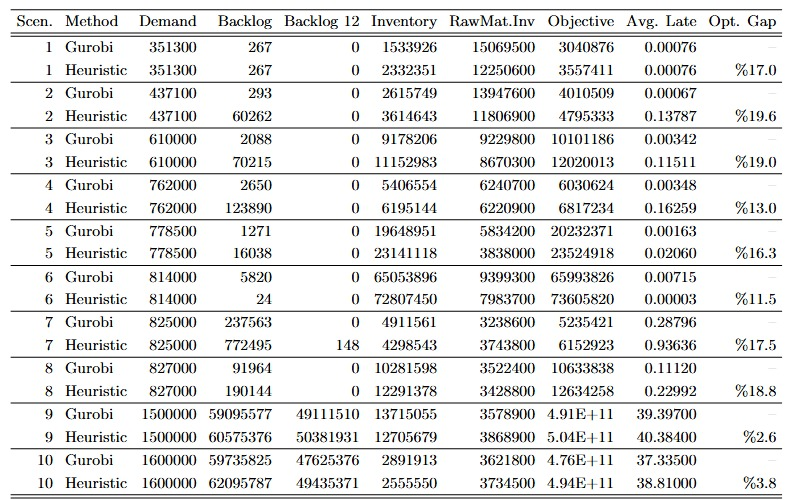
\includegraphics[width=1\linewidth]{figures/fig5.jpg}
    \caption{Comparison between mathematical model and heuristic approach}
    \label{fig:mha}
\end{figure}
\subsubsection{Verification of the Stochastic Solution Approach}

Since the two-stage stochastic solution approach is only implemented on the long-term mathematical model, the verification of this implementation has been done by conducting a logical comparison with the deterministic approach, changing the stochasticity parameters, conducting a $VSS$ (Value of Stochastic Solution) computation, and examining the output of the hierarchical decision support system after implementation. First, an output comparison between the deterministic and the stochastic long-term model was made. Both models had been run with the same demand parameters, with only one scenario available (original demand scenario) in the stochastic model. Final outputs of both models showed exactly the same resulting inventory and production decisions. 

Then, a $VSS$ analysis was conducted to measure the benefit of using the stochastic solution approach. The Value of the Stochastic Solution was formally introduced by \cite{birge1982vss} for stochastic linear programs with fixed recourse and is the standard metric for quantifying the cost penalty of ignoring uncertainty in two-stage formulations. First, the full-horizon stochastic model (Recourse Problem) was solved to obtain the stochastic objective value, in which demand uncertainty was represented by a set of 10 possible scenarios with 15\% variance. Then, the corresponding expected value (EV) model was constructed by replacing uncertain demand parameters with their expected values and solving this deterministic approximation. The solution obtained from the EV model was evaluated under the original stochastic model to compute the expected result of the expected-value solution (EEV). For this project's minimization problem, the $VSS$ is calculated as

\[
VSS = EEV - RP
\]

where \(RP\) denotes the optimal objective value of the stochastic recourse problem, and \(EEV\) denotes the expected performance of the expected-value solution under uncertainty. These calculations were made for 100 different iterations by changing the demand parameter structure randomly (25\% variance from the original demand setup). As a result, the benefit of using a stochastic solution approach has been proven by obtaining non-negative $VSS$ for each iteration. Also, $VSS$ analysis shows that the average objective value of the stochastic model solution is significantly lower due to high demand uncertainty and enormous backlog costs. The VSS analysis results, which are made by 100 iterations, are shown in the table \ref{tab:vss} below.


\begin{table}[h!]
\caption{VSS analysis results}
\label{tab:vss}
\centering

\begin{tabular}{|l |l |l|}\hline   
Average $RP$ Objective Value& \multicolumn{2}{|l|}{4,454,400} \\\hline
Average $EEV$ Objective Value& \multicolumn{2}{|l|}{41,626,235} \\\hline
Average $VSS$ ($EEV - RP$)& \multicolumn{2}{|l|}{37,171,834} \\\hline
Average $VSS$ (avg of \%)& \multicolumn{2}{|l|}{80.48\%} \\\hline
Min $VSS$& \multicolumn{2}{|l|}{0.00} \\\hline
Max $VSS$& \multicolumn{2}{|l|}{87,435,901} \\\hline

\end{tabular}

\end{table}




After this phase, both deterministic and stochastic solution approaches had been tested with the yearly rolling horizon methodology. The logical expectation for the outputs of the stochastic solution approach had been successfully satisfied. The stochastic model had been run with ten scenarios generated from the initial forecast, with a maximum 15\% variance from the initial forecast. The stochastic model generated a higher amount of inventory decisions on a yearly basis. The reason for this output was that under the uncertainty of demand, the probability of facing a greater demand than expected generates a huge amount of risk due to the enormous backlog costs. The model tries to lower the risk of these possible backlogs in the future by keeping more products in the inventory, which increases the total holding cost of the stochastic model. In the end, when both models face differences between the forecast and the realized demand, the stochastic model generates an inventory plan with lower total cost, lower backlog cost, and a higher holding cost, as shown in table \ref{tab.rhvss}. 


\begin{table}[h!]
\caption{Cost comparisons of stochastic and deterministic models}
\label{tab.rhvss}
\centering

\begin{tabular}{l l l l}\toprule
& Stochastic& Deterministic& Difference\\\midrule
Avg. Holding Cost& 5,634,045 & 2,901,458 & -2,732,587 \\
Avg. Backlog Cost& 48,057,008 & 89,656,018 & 41,599,010 \\
Avg. Total Cost & 53,691,052 & 92,557,476 & 38,866,424 \\ \bottomrule

\end{tabular}

\end{table}


 Also, changing stochastic parameters, such as the number of scenarios and the deviation between these scenarios, showed logical results. The model had run with changing the number of scenarios from five to twenty, and changing the variance between 5\% to 25\%. Adjusting different demand variances for scenarios caused higher uncertainty in the model, which resulted in higher inventory decisions and holding costs. The weight of the worst-case scenarios on the inventory decisions is heavy, due to huge backlog costs. In conclusion, the verification step of the stochastic solution approach has shown logical results for each case and has also been implemented successfully on our solution approach. 

\subsection{Validation}
In the validation phase, real company input data and forecast structures were used to run the rolling horizon decision support system over the planning horizon. The purpose of this phase was to evaluate whether the outputs of the proposed long-term and short-term planning structure are compatible with the company’s production environment and operational priorities. The outputs were analyzed in terms of demand satisfaction, backlog behavior, inventory build-ahead decisions, and consistency with the company’s production structure. In this sense, the validation study mainly relies on expert opinion and output-based operational validity, rather than a full pilot implementation.

The analysis showed that the model behaves in a way that is consistent with the company’s planning logic and business needs. During peak demand periods, the system builds inventory ahead and uses this inventory to reduce the risk of excessive backlog in later periods. This behavior was found to be aligned with the company’s description of a desirable planning approach. In addition, the raw material side of the system was modeled with a policy-based mechanism rather than full short-term optimization for all materials. This modeling choice was made due to the limited short-term planning horizon and was explicitly recommended by the industrial advisor as a practical and efficient way to represent procurement behavior within the current project scope.

Another important validation outcome is that the rolling horizon structure can adapt to forecast updates during the year. When updated forecasts decrease, the model correspondingly reduces build-ahead and production levels to avoid unnecessary inventory accumulation. When updated forecasts increase, the model tries to respond by using all available planning flexibility, including available capacity and previously built inventory, in order to keep backlog under control. According to the feedback received from the industrial advisor, this adaptive behavior is both realistic and operationally desirable for the company. Therefore, the validation results support that the proposed decision support system is a credible representation of the planning problem and that its outputs are suitable for practical use in the company environment.

Figure \ref{fig:valid}, which shows the yearly evolution of production-demand balance can be used to further support this validation. This visualization helps to demonstrate that the model output not only remains feasible but also follows a planning pattern that is interpretable and consistent with company practice.

\begin{figure}[h!]
    \centering
    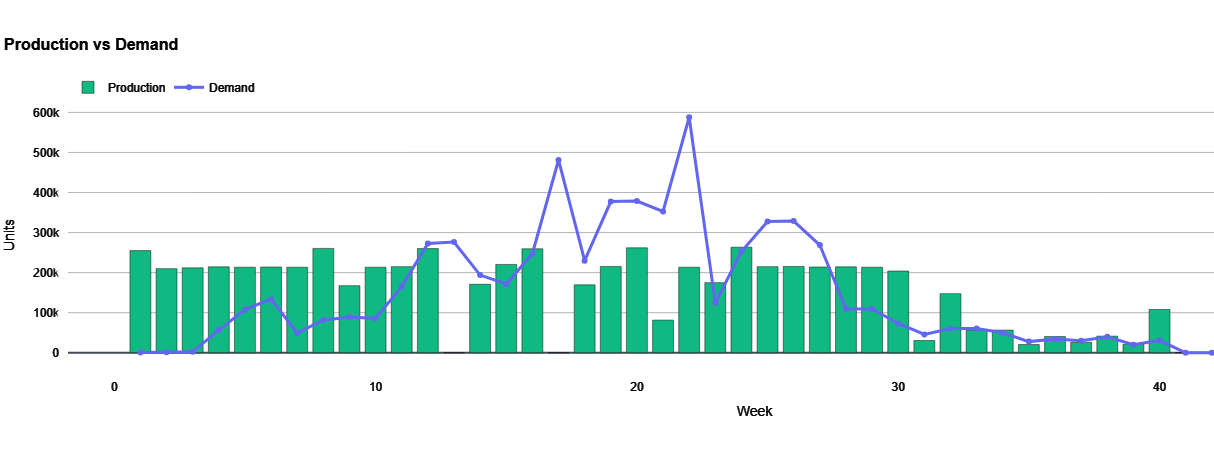
\includegraphics[width=1\linewidth]{figures/prodem.png}
    \caption{Production and Demand Levels Throughout the Year}
    \label{fig:valid}
\end{figure}



\section{Outcome and Deliverables}
\subsection{Outcome}
The outcome of this project is a decision support system that delivers quantitative production and inventory plans for Nesco’s BobaCo brand. The system generates results over the entire planning horizon, including daily production decisions for each product and optimized inventory levels for both semi-finished and finished goods. It specifies how much inventory should be built up in advance to prepare for seasonal demand and reports the raw material quantities required to support the planned production. Overall, the outcome is a comprehensive planning tool that links monthly and daily decisions, ensuring feasible, balanced, and well-organized production and inventory plans for BobaCo’s operations.\\

\subsection{Deliverables}

The main deliverable of this project is a decision support system that coordinates BobaCo’s production and inventory planning. This system is built around an integrated optimization model that determines monthly output levels, daily production schedules, and inventory levels over the planning horizon. The model explicitly accounts for capacity limits, seasonal demand patterns, line-specific constraints, and product shelf life. Based on the resulting plan, the system also computes the required raw material quantities implied by the planned production levels.\ 

\indent Since the integrated model cannot be solved to optimality within a reasonable computation time, the decision support system employs a hierarchical heuristic embedded in the same interface. This heuristic approximates the model by decomposing it into a long-term planning step that sets monthly production and inventory targets and a short-term scheduling step that translates these targets into feasible daily production plans on each line. Thus, the long-term and short-term structure is used as the solution approach. Furthermore, to address demand uncertainty, the long-term tier integrates a two-stage stochastic programming formulation that evaluates multiple demand scenarios generated from a base forecast.

\indent The system has been successfully developed as a Python-based software application, the Weekly Planner. This tool accepts user inputs via a web-based interface built with Streamlit and uses historical sales data and capacity constraints defined in Excel spreadsheets. Python optimization scripts process this data to produce actionable production and inventory planning results. Output is displayed dynamically through interactive charts and data tables, ensuring the system can perform the core tasks of accepting inputs, running the optimization models, and clearly presenting the outputs to the planners.\ 

\indent In practice, users configure the expected demand forecasts, capacities, cost parameters, and uncertainty bounds through the application sidebar. Inputs can be updated on a rolling basis; long-term parameters are typically revised monthly, and short-term data is updated weekly. The decision support system then generates the optimal aggregate production and inventory plans, along with detailed daily production line assignments and period-by-period raw material requirement orders. For archival and reporting, all tabular results can be exported directly to detailed multi-sheet Excel files.\ 

\indent Finally, the software suite is accompanied by a comprehensive User Manual. This manual provides detailed, step-by-step instructions with interface screenshots on how to configure and execute the Weekly Planner application. It specifies how to interpret the model outputs, update parameters for the rolling horizon, and apply the stochastic planning tools intuitively. This combined package ensures the company can deploy the deliverable into their operations and utilize it effectively during the upcoming pilot study and future planning cycles.

\indent The prototype of the user interface, the user manual for the UI, and the input template, which will be used for the decision support system, can be seen in Appendix \ref{sec:first-app}.\\

\subsection{Benchmarking and Benefits to the Company}

After completing the validation phase, a benchmarking analysis was conducted to compare the proposed decision support system with the company’s current planning approach under the same demand inputs. In this comparison, the current system was approximated by a 35-day backward allocation rule. Since the company reacts to delays exceeding 12 days by using overtime, the benchmarking mainly focuses on KPIs related to backlog risk and overtime dependency.

The following KPIs were used in the comparison:

\begin{itemize}
    \item \textbf{Backlogs Under Cancellation Risk}: This KPI records the amount of backlog that exceeds 12 days. Since such delays are operationally critical for the company, reducing this amount is one of the main targets of the proposed system.
\end{itemize}
\begin{itemize}
    \item \textbf{Overtime Days}: This KPI measures the number of days on which overtime production is required. It directly shows how much the planning approach depends on reactive capacity usage.
\end{itemize}
\begin{itemize}
    \item \textbf{Overtime Delivery Rate}: This KPI measures the share of total demand that must be recovered through overtime-related production. It is used to quantify how much of total yearly demand cannot be handled within regular capacity.

\end{itemize}

Under the original 2026 forecast, the current system required 11 overtime days and created 380,709 units of backlog under cancellation risk out of a total demand of 6,330,210 units, corresponding to an overtime-related delivery rate of 6.01\%. Under the same forecast, the proposed system eliminated this need completely and produced no residual backlog.

To test the robustness of the proposed system under uncertainty, 10 additional demand scenarios were generated around the same monthly forecast. In these scenarios, monthly product-level demand totals were allowed to deviate by at most 25\% from the forecast, and the corresponding demand was randomly distributed across the working days of each month. This allowed the benchmarking process to evaluate the planning systems under a wider range of possible yearly demand realizations instead of relying only on a single forecast path.

Across these 10 scenarios, the current system required between 17 and 37 overtime days, with an average of 28.2 days, and created a total of 8,082,588 units of backlog under cancellation risk over 64,721,203 units of total demand, corresponding to a weighted risk ratio of 12.49\%. In contrast, the proposed system achieved zero backlog and zero overtime in 7 of the 10 scenarios. In the remaining 3 scenarios, it required only 1 overtime day and created only limited residual backlog. Across all 10 scenarios, the proposed system’s average overtime requirement was 0.3 days, and its total remaining backlog was only 49,330 units, corresponding to a ratio of 0.08\% of total demand.

These findings show that the company’s current planning logic is highly sensitive to demand fluctuations and frequently requires reactive overtime to recover delayed orders. The proposed rolling-horizon decision support system performs much more robustly by building inventory ahead when necessary and by reducing the accumulation of backlog beyond the 12-day tolerance window. Therefore, the main benefit to the company is not only a reduction in backlog risk, but also a substantial reduction in overtime dependency under both the base forecast and the generated demand scenarios. Since raw material shortage based infeasibilities were excluded from this comparison, the reported improvement should be interpreted specifically as the benefit of better production planning and proactive inventory build-ahead.

\begin{table}[h!]
\centering
\caption{Benchmarking Results for the Current and Proposed Systems}
\label{tab:benchmark_results}
\renewcommand{\arraystretch}{1.2}
\begin{tabular}{|p{5.8cm}|c|c|}
\hline
\textbf{Metric} & \textbf{Current System} & \textbf{Proposed System} \\ \hline
Base-case overtime days & 11 & 0 \\ \hline
Base-case overtime-dependent volume & 380,709 & 0 \\ \hline
Base-case overtime delivery rate & 6.01\% & 0.00\% \\ \hline
Average overtime days across 10 scenarios & 28.2 & 0.3 \\ \hline
Range of overtime days across scenarios & 17--37 & 0--1 \\ \hline
Weighted overtime-related / delayed volume ratio & 12.49\% & 0.08\% \\ \hline
Scenarios with zero backlog and zero overtime & 0/10 & 7/10 \\ \hline
\end{tabular}
\end{table}

\subsection{Implementation and Pilot Study}

The decision support system was integrated into the company’s weekly production planning process through a structured four-week pilot study. The main objective of the pilot was to measure how much of the upcoming months’ forecasted demand can be proactively converted into inventory through the planning decisions generated by the system. To support evaluation during the pilot period, a simple weekly inventory snapshot routine was used to record starting inventory levels and monitor inventory evolution over time. At the end of the pilot period, results were summarized based on the weekly decision logs and inventory observations, focusing on inventory coverage progress, practicality of the recommended plans, and integration into the weekly planning routine. These findings guided the final refinements and support the transition toward sustained operational use.


\indent In coordination with company representatives, an interface was developed in line with the firm’s existing reporting practices, which facilitated adoption by planners. Figure \ref{fig:weekly_output} presents the user interface of the decision support system together with a sample weekly production schedule generated by the system. The first week was conducted under the close supervision of the project team, while the following weeks were carried out directly by the company within its regular planning routine. On a weekly basis, the tool generated recommended production quantities and raw material order decisions based on updated demand information and current operational inputs. These recommendations were reviewed every Monday for feasibility and shop-floor consistency, and the finalized plans and manual adjustments were documented in weekly decision records.

\begin{figure}[h!]
    \centering
    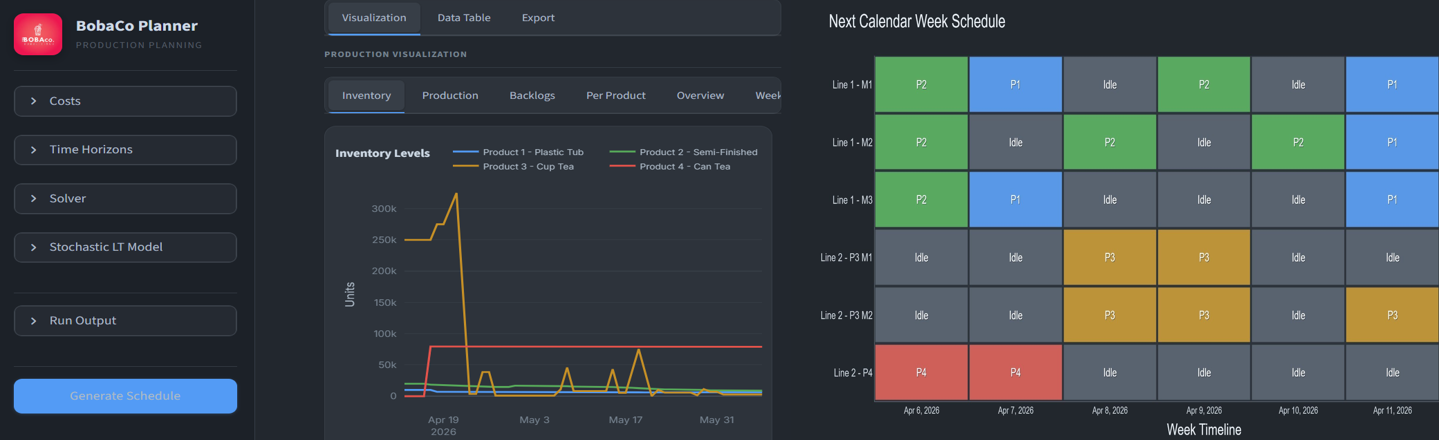
\includegraphics[width=1.04\linewidth]{figures/Ui_and_Wschedule.png}
    \caption{System interface and sample weekly schedule output.}
    \label{fig:weekly_output}
\end{figure}

During the pilot study, the decision support system generated weekly production plans in a consistent and operationally interpretable manner. The company reviewed these recommendations each week and approved them as feasible for its regular planning process. In some weeks, the system recommended producing slightly more than the company’s immediate production plan and holding the excess quantity as inventory. Although the pilot study period did not fully coincide with the peak-demand season, the company considered this behavior positive because it reflected the project's main purpose: preparing for future demand increases through proactive inventory build-ahead. Therefore, the pilot study did not directly measure the full peak-season impact of the system, but it confirmed that the model’s weekly decisions were understandable, feasible, and consistent with the company’s objective of using available capacity to prepare for high-demand periods.

\section{Conclusion and Future Work}

The project met the company’s expectations by developing a decision support system that improves production planning under seasonal and uncertain demand. The proposed structure combines hierarchical production planning, a stochastic long-term model, a short-term production planning model, and a rolling-horizon mechanism to produce plans that are both operationally feasible and responsive to changing conditions. The validation results showed that the system supports proactive inventory build-ahead and reacts quickly to forecast updates and changes in available workdays. In addition, the yearly rolling-horizon implementation results indicated that the stochastic approach provides a more robust balance between inventory protection and backlog risk under uncertainty, reducing the average total cost by 42.0\%. This relatively great improvement is mainly due to the model structure, where backlog costs are much higher than holding costs, so carrying additional inventory helps avoid much larger backlog-related losses.

The practical value of the system was also demonstrated through benchmarking and pilot use. Compared with the company’s current planning logic, the proposed approach substantially reduced overtime dependency, lowering average overtime requirement from 28.2 days to 0.3 days and achieving zero backlog and zero overtime in 7 out of 10 generated demand scenarios. In addition, the four-week pilot study showed that the system could be incorporated into the company’s weekly planning routine and could support inventory positioning for the high demand anticipated in the 2026 summer forecast. Future work may focus on improving the scenario generation structure through observations collected over longer periods, allowing demand uncertainty to be represented in an even more realistic way. 

% if there is only one appendix, use \appendix[<title of appendix>] and \subsection* if needed
\appendix
\section{Appendix User Interface }
\label{sec:first-app}
\begin{figure}[h!]
    \centering
    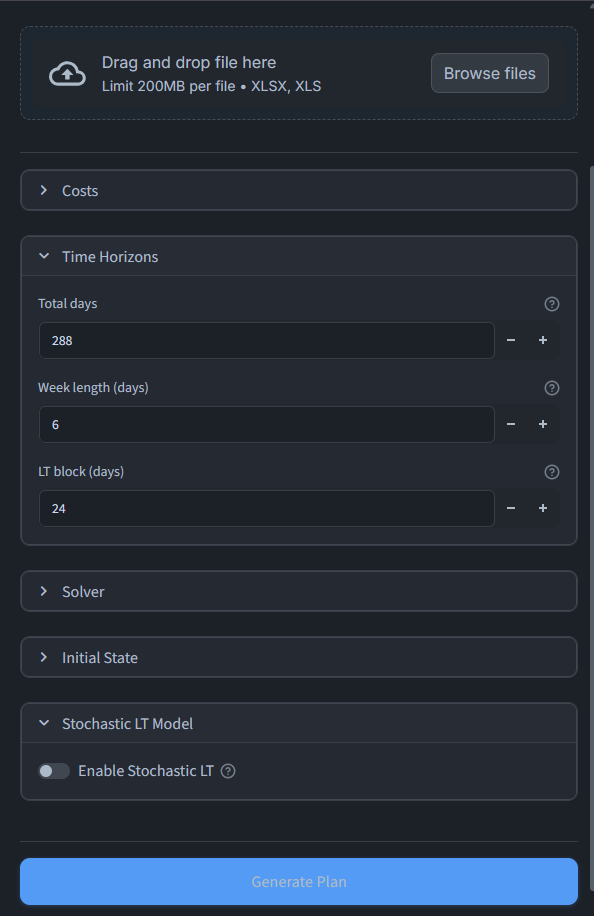
\includegraphics[width=0.75\linewidth]{figures/UI.png}
    \caption{The Input Field of the User Interface}
    \label{fig:placeholder}
\end{figure}
\begin{figure}[h!]
    \centering
    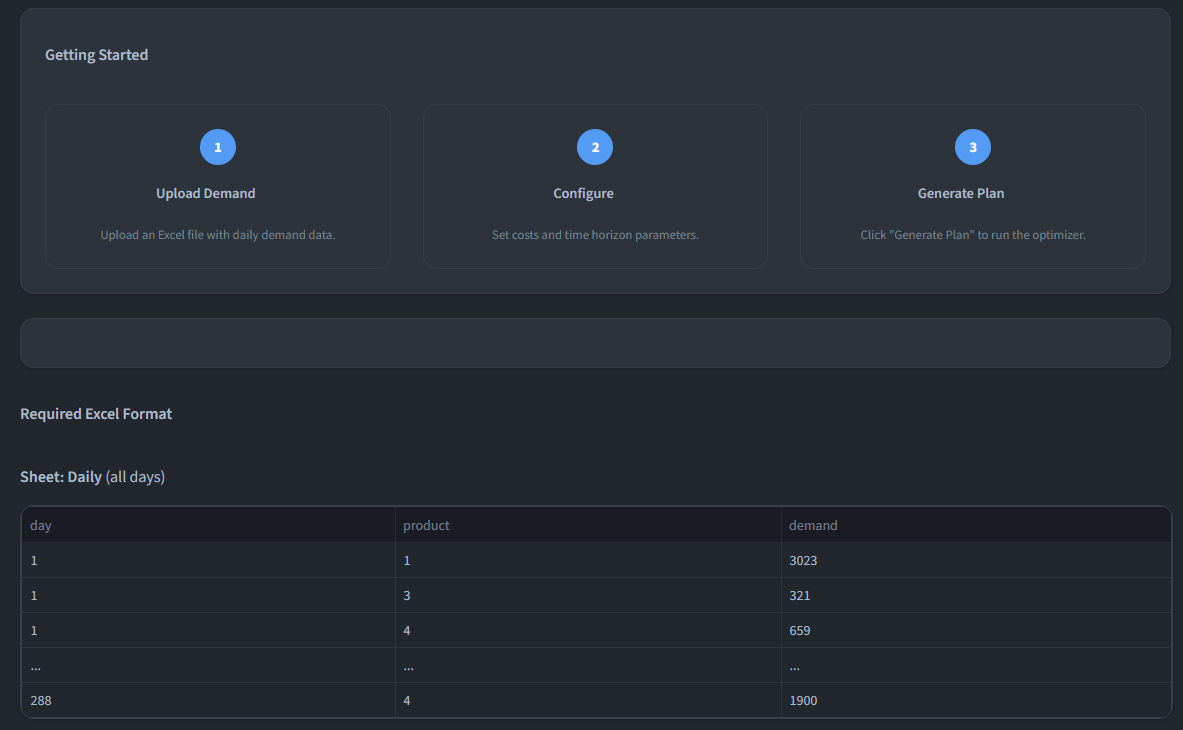
\includegraphics[width=1\linewidth]{figures/UIMAN.png}
    \caption{The User Interface Manual}
    \label{fig:placeholder}
\end{figure}

\begin{figure}[h!]
    \centering
    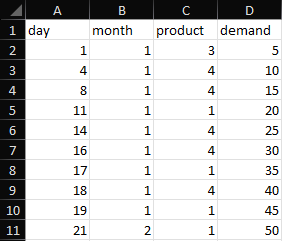
\includegraphics[width=0.5\linewidth]{figures/input.png}
    \caption{An artificial example of an Excel input template needed for the decision support system}
    \label{fig:placeholder}
\end{figure}


\begin{figure}[h!]
    \centering
    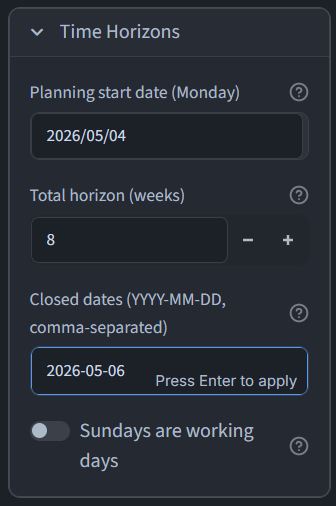
\includegraphics[width=0.75\linewidth]{figures/workdays.png}
    \caption{Time horizon configuration panel of the decision support interface }
    \label{fig:placeholder}
\end{figure}


\begin{figure}[h!]
    \centering
    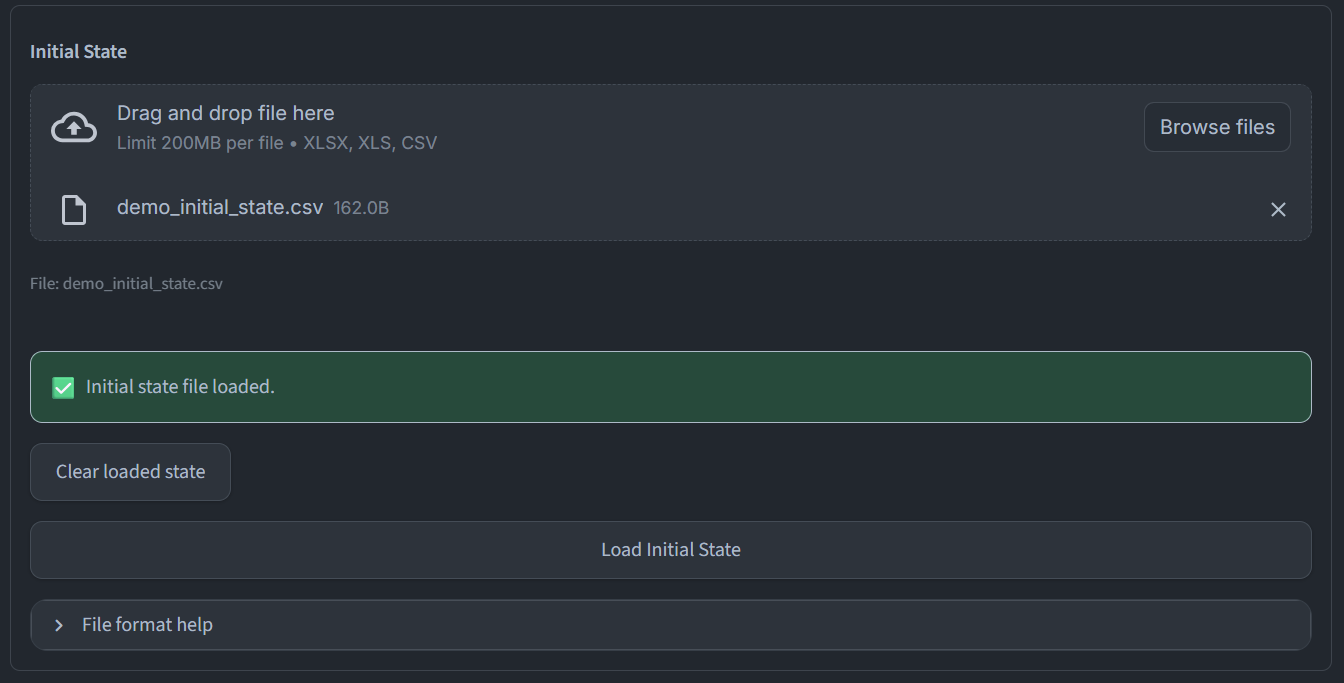
\includegraphics[width=1\linewidth]{figures/file upload.png}
    \caption{Initial state upload panel of the decision support interface }
    \label{fig:placeholder}
\end{figure}

\begin{figure}[h!]
    \centering
    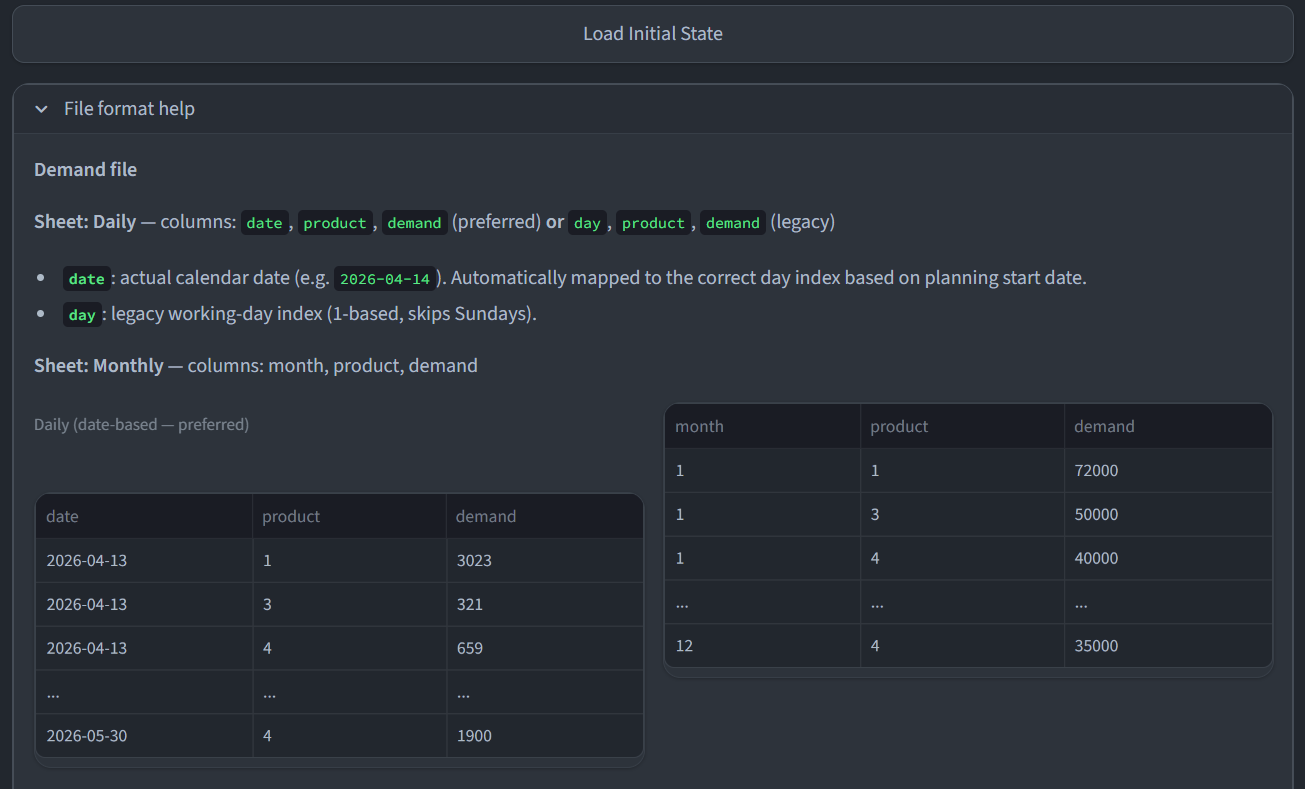
\includegraphics[width=1\linewidth]{figures/file format help.png}
    \caption{File upload manual}
    \label{fig:placeholder}
\end{figure}

\end{document}

